%%%%%%%%%%%%%%%%%%%%%%%%%%%%%%%%%%%%%%%%%%%%%%%%%%%%%
% settings                                          %
%                                                   %
% einbinden mit: %%%%%%%%%%%%%%%%%%%%%%%%%%%%%%%%%%%%%%%%%%%%%%%%%%%%%
% settings                                          %
%                                                   %
% einbinden mit: %%%%%%%%%%%%%%%%%%%%%%%%%%%%%%%%%%%%%%%%%%%%%%%%%%%%%
% settings                                          %
%                                                   %
% einbinden mit: \input{settings}                   %
%%%%%%%%%%%%%%%%%%%%%%%%%%%%%%%%%%%%%%%%%%%%%%%%%%%%%

\documentclass[a4paper, 11pt, oneside, openany,abstracton]{scrreprt} % koma-script layout

% --------------------------------------
% alle packages die wir brauchen:
% --------------------------------------

% Schriften, Sprache, Text:
\usepackage[T1]{fontenc}
\usepackage[latin1]{inputenc}
%\usepackage[german]{babel}
%\usepackage{../tex-include/german} %sonst gehen die Anfhrungzeichen nicht!
%\usepackage{../tex-include/ngerman}
%\usepackage[english]{babel}
%\usepackage{english}

\usepackage[T1]{fontenc}
\usepackage[scaled]{../tex-include/uarial}
\renewcommand*\familydefault{\sfdefault} %% Only if the base font of the document is to be sans serif

\usepackage{hyperref}
\usepackage{../tex-include/glossaries}
\makeglossaries

\usepackage{pifont}
\newcommand{\tick}{\quad\quad\color{green}{\ding{52}}}
\newcommand{\partialTick}{\quad\quad\color{green}{(\ding{52})}}
\newcommand{\cross}{\quad\quad\color{red}{\ding{54}}}

\usepackage{pdfpages}


% wegen deutschen Umlauten
%\usepackage[ansinew]{inputenc}
% alles in Farbe:
\usepackage{color}
\usepackage{listings}
\lstset{ %
language=C,                		% choose the language of the code
basicstyle=\footnotesize,       % the size of the fonts that are used for the code
frame=single,			% adds a frame around the code
captionpos=b,			% sets the caption-position to bottom
breaklines=true,		% sets automatic line breaking
breakatwhitespace=false,	% sets if automatic breaks should only happen at whitespace
tabsize=2,
escapeinside={\%*}{*)}          % if you want to add a comment within your code
}

% Tabellen
\usepackage{tabularx}
\usepackage{../tex-include/multirow}
\usepackage{multicol}
\usepackage{longtable}
\usepackage{hhline}
\usepackage{booktabs}
% Boxen
\usepackage{../tex-include/pbox} 
% Aufzaehlungen
\usepackage{../tex-include/shortlst}
% Equation array mit mehrfacher Ausrichtung
\usepackage{array}
% verbatim
\usepackage{fancyvrb}
% Grafik:
\usepackage{epsfig}
\usepackage{../tex-include/texdraw}
\usepackage{graphicx}
\usepackage{flafter}
\usepackage[bf]{caption2}  % Wort Abbildung bold
\usepackage{float} % grafik genau hier einbinden mit [H]
% AMS-Math:
\usepackage{amsmath}
\usepackage{amstext}
\usepackage{amstext}
\usepackage{amsfonts}
\usepackage{amsxtra}
\usepackage{amssymb}
%\usepackage{../tex-include/stmaryrd} % blitz
\usepackage{../tex-include/wasysym}  % varangle
% double Stroke Fonts
\usepackage{../tex-include/bbm}
% Index, Headers
\usepackage{makeidx}
\usepackage{fancyhdr}
\usepackage{lscape}
\usepackage{enumerate}
% Schrift fr PDF wegen [T1]
\usepackage{ae,aecompl}



%\usepackage{hyperref}
% \usepackage[
%   colorlinks,
%   linkcolor=blue,
%   urlcolor=red%
% ]{hyperref}

\usepackage{color}
\definecolor{darkblue}{rgb}{0,0.1,0.5}
\hypersetup{colorlinks,
            linkcolor=darkblue,
            anchorcolor=darkblue,
            citecolor=darkblue}

%\definecolor{darkblue}{rgb}{0,0.1,0.5}
\hypersetup{pdftex=true, colorlinks=false, breaklinks=true, linkcolor=darkblue, menucolor=darkblue, pagecolor=darkblue, urlcolor=darkblue}

% Zum Programmieren
\usepackage{ifthen}
\usepackage{calc}
%struktogramme erstellen


%-------------------------
% Bibliography, index
%-------------------------
% fuer Zitate
\usepackage[square]{natbib}

% Festlegung Art der Zitierung - Havardmethode: Abkuerzung Autor + Jahr
%\bibliographystyle{IEEEtranSA}
\bibliographystyle{plain}

% Stichwortverzeichnis erstellen
%\makeindex

% --------------------------------------
% Seitenraender neu einstellen:
% --------------------------------------

% einstellungen r�der fuer caption2
\setcaptionwidth{0.8\textwidth}


%einstellungen fr list umgebung
\setlength{\topsep}{0pt}
\setlength{\itemsep}{0.2pt}
\setlength{\parsep}{0pt}

%einstellungen fr seitenlayout
\setlength{\marginparwidth}{0pt}
\setlength{\textwidth}{440pt}
\setlength{\hoffset}{-20pt}
\setlength{\voffset}{-20pt}
\setlength{\evensidemargin}{0pt}
\setlength{\topmargin}{0pt}
\setlength{\headheight}{14pt}
\setlength{\headsep}{18pt}
\setlength{\textheight}{670pt}
\setlength{\marginparsep}{0pt}
\setlength{\marginparpush}{5pt}
\setlength{\footskip}{27pt}



% --------------------------------------
% Einstellungen fr das Koma Skript
% --------------------------------------

% weniger leerraum ber dem chapter titel
\renewcommand*{\chapterheadstartvskip}{\vspace*{-1cm}}



                   %
%%%%%%%%%%%%%%%%%%%%%%%%%%%%%%%%%%%%%%%%%%%%%%%%%%%%%

\documentclass[a4paper, 11pt, oneside, openany,abstracton]{scrreprt} % koma-script layout

% --------------------------------------
% alle packages die wir brauchen:
% --------------------------------------

% Schriften, Sprache, Text:
\usepackage[T1]{fontenc}
\usepackage[latin1]{inputenc}
%\usepackage[german]{babel}
%\usepackage{../tex-include/german} %sonst gehen die Anfhrungzeichen nicht!
%\usepackage{../tex-include/ngerman}
%\usepackage[english]{babel}
%\usepackage{english}

\usepackage[T1]{fontenc}
\usepackage[scaled]{../tex-include/uarial}
\renewcommand*\familydefault{\sfdefault} %% Only if the base font of the document is to be sans serif

\usepackage{hyperref}
\usepackage{../tex-include/glossaries}
\makeglossaries

\usepackage{pifont}
\newcommand{\tick}{\quad\quad\color{green}{\ding{52}}}
\newcommand{\partialTick}{\quad\quad\color{green}{(\ding{52})}}
\newcommand{\cross}{\quad\quad\color{red}{\ding{54}}}

\usepackage{pdfpages}


% wegen deutschen Umlauten
%\usepackage[ansinew]{inputenc}
% alles in Farbe:
\usepackage{color}
\usepackage{listings}
\lstset{ %
language=C,                		% choose the language of the code
basicstyle=\footnotesize,       % the size of the fonts that are used for the code
frame=single,			% adds a frame around the code
captionpos=b,			% sets the caption-position to bottom
breaklines=true,		% sets automatic line breaking
breakatwhitespace=false,	% sets if automatic breaks should only happen at whitespace
tabsize=2,
escapeinside={\%*}{*)}          % if you want to add a comment within your code
}

% Tabellen
\usepackage{tabularx}
\usepackage{../tex-include/multirow}
\usepackage{multicol}
\usepackage{longtable}
\usepackage{hhline}
\usepackage{booktabs}
% Boxen
\usepackage{../tex-include/pbox} 
% Aufzaehlungen
\usepackage{../tex-include/shortlst}
% Equation array mit mehrfacher Ausrichtung
\usepackage{array}
% verbatim
\usepackage{fancyvrb}
% Grafik:
\usepackage{epsfig}
\usepackage{../tex-include/texdraw}
\usepackage{graphicx}
\usepackage{flafter}
\usepackage[bf]{caption2}  % Wort Abbildung bold
\usepackage{float} % grafik genau hier einbinden mit [H]
% AMS-Math:
\usepackage{amsmath}
\usepackage{amstext}
\usepackage{amstext}
\usepackage{amsfonts}
\usepackage{amsxtra}
\usepackage{amssymb}
%\usepackage{../tex-include/stmaryrd} % blitz
\usepackage{../tex-include/wasysym}  % varangle
% double Stroke Fonts
\usepackage{../tex-include/bbm}
% Index, Headers
\usepackage{makeidx}
\usepackage{fancyhdr}
\usepackage{lscape}
\usepackage{enumerate}
% Schrift fr PDF wegen [T1]
\usepackage{ae,aecompl}



%\usepackage{hyperref}
% \usepackage[
%   colorlinks,
%   linkcolor=blue,
%   urlcolor=red%
% ]{hyperref}

\usepackage{color}
\definecolor{darkblue}{rgb}{0,0.1,0.5}
\hypersetup{colorlinks,
            linkcolor=darkblue,
            anchorcolor=darkblue,
            citecolor=darkblue}

%\definecolor{darkblue}{rgb}{0,0.1,0.5}
\hypersetup{pdftex=true, colorlinks=false, breaklinks=true, linkcolor=darkblue, menucolor=darkblue, pagecolor=darkblue, urlcolor=darkblue}

% Zum Programmieren
\usepackage{ifthen}
\usepackage{calc}
%struktogramme erstellen


%-------------------------
% Bibliography, index
%-------------------------
% fuer Zitate
\usepackage[square]{natbib}

% Festlegung Art der Zitierung - Havardmethode: Abkuerzung Autor + Jahr
%\bibliographystyle{IEEEtranSA}
\bibliographystyle{plain}

% Stichwortverzeichnis erstellen
%\makeindex

% --------------------------------------
% Seitenraender neu einstellen:
% --------------------------------------

% einstellungen r�der fuer caption2
\setcaptionwidth{0.8\textwidth}


%einstellungen fr list umgebung
\setlength{\topsep}{0pt}
\setlength{\itemsep}{0.2pt}
\setlength{\parsep}{0pt}

%einstellungen fr seitenlayout
\setlength{\marginparwidth}{0pt}
\setlength{\textwidth}{440pt}
\setlength{\hoffset}{-20pt}
\setlength{\voffset}{-20pt}
\setlength{\evensidemargin}{0pt}
\setlength{\topmargin}{0pt}
\setlength{\headheight}{14pt}
\setlength{\headsep}{18pt}
\setlength{\textheight}{670pt}
\setlength{\marginparsep}{0pt}
\setlength{\marginparpush}{5pt}
\setlength{\footskip}{27pt}



% --------------------------------------
% Einstellungen fr das Koma Skript
% --------------------------------------

% weniger leerraum ber dem chapter titel
\renewcommand*{\chapterheadstartvskip}{\vspace*{-1cm}}



                   %
%%%%%%%%%%%%%%%%%%%%%%%%%%%%%%%%%%%%%%%%%%%%%%%%%%%%%

\documentclass[a4paper, 11pt, oneside, openany,abstracton]{scrreprt} % koma-script layout

% --------------------------------------
% alle packages die wir brauchen:
% --------------------------------------

% Schriften, Sprache, Text:
\usepackage[T1]{fontenc}
\usepackage[latin1]{inputenc}
%\usepackage[german]{babel}
%\usepackage{../tex-include/german} %sonst gehen die Anfhrungzeichen nicht!
%\usepackage{../tex-include/ngerman}
%\usepackage[english]{babel}
%\usepackage{english}

\usepackage[T1]{fontenc}
\usepackage[scaled]{../tex-include/uarial}
\renewcommand*\familydefault{\sfdefault} %% Only if the base font of the document is to be sans serif

\usepackage{hyperref}
\usepackage{../tex-include/glossaries}
\makeglossaries

\usepackage{pifont}
\newcommand{\tick}{\quad\quad\color{green}{\ding{52}}}
\newcommand{\partialTick}{\quad\quad\color{green}{(\ding{52})}}
\newcommand{\cross}{\quad\quad\color{red}{\ding{54}}}

\usepackage{pdfpages}


% wegen deutschen Umlauten
%\usepackage[ansinew]{inputenc}
% alles in Farbe:
\usepackage{color}
\usepackage{listings}
\lstset{ %
language=C,                		% choose the language of the code
basicstyle=\footnotesize,       % the size of the fonts that are used for the code
frame=single,			% adds a frame around the code
captionpos=b,			% sets the caption-position to bottom
breaklines=true,		% sets automatic line breaking
breakatwhitespace=false,	% sets if automatic breaks should only happen at whitespace
tabsize=2,
escapeinside={\%*}{*)}          % if you want to add a comment within your code
}

% Tabellen
\usepackage{tabularx}
\usepackage{../tex-include/multirow}
\usepackage{multicol}
\usepackage{longtable}
\usepackage{hhline}
\usepackage{booktabs}
% Boxen
\usepackage{../tex-include/pbox} 
% Aufzaehlungen
\usepackage{../tex-include/shortlst}
% Equation array mit mehrfacher Ausrichtung
\usepackage{array}
% verbatim
\usepackage{fancyvrb}
% Grafik:
\usepackage{epsfig}
\usepackage{../tex-include/texdraw}
\usepackage{graphicx}
\usepackage{flafter}
\usepackage[bf]{caption2}  % Wort Abbildung bold
\usepackage{float} % grafik genau hier einbinden mit [H]
% AMS-Math:
\usepackage{amsmath}
\usepackage{amstext}
\usepackage{amstext}
\usepackage{amsfonts}
\usepackage{amsxtra}
\usepackage{amssymb}
%\usepackage{../tex-include/stmaryrd} % blitz
\usepackage{../tex-include/wasysym}  % varangle
% double Stroke Fonts
\usepackage{../tex-include/bbm}
% Index, Headers
\usepackage{makeidx}
\usepackage{fancyhdr}
\usepackage{lscape}
\usepackage{enumerate}
% Schrift fr PDF wegen [T1]
\usepackage{ae,aecompl}



%\usepackage{hyperref}
% \usepackage[
%   colorlinks,
%   linkcolor=blue,
%   urlcolor=red%
% ]{hyperref}

\usepackage{color}
\definecolor{darkblue}{rgb}{0,0.1,0.5}
\hypersetup{colorlinks,
            linkcolor=darkblue,
            anchorcolor=darkblue,
            citecolor=darkblue}

%\definecolor{darkblue}{rgb}{0,0.1,0.5}
\hypersetup{pdftex=true, colorlinks=false, breaklinks=true, linkcolor=darkblue, menucolor=darkblue, pagecolor=darkblue, urlcolor=darkblue}

% Zum Programmieren
\usepackage{ifthen}
\usepackage{calc}
%struktogramme erstellen


%-------------------------
% Bibliography, index
%-------------------------
% fuer Zitate
\usepackage[square]{natbib}

% Festlegung Art der Zitierung - Havardmethode: Abkuerzung Autor + Jahr
%\bibliographystyle{IEEEtranSA}
\bibliographystyle{plain}

% Stichwortverzeichnis erstellen
%\makeindex

% --------------------------------------
% Seitenraender neu einstellen:
% --------------------------------------

% einstellungen r�der fuer caption2
\setcaptionwidth{0.8\textwidth}


%einstellungen fr list umgebung
\setlength{\topsep}{0pt}
\setlength{\itemsep}{0.2pt}
\setlength{\parsep}{0pt}

%einstellungen fr seitenlayout
\setlength{\marginparwidth}{0pt}
\setlength{\textwidth}{440pt}
\setlength{\hoffset}{-20pt}
\setlength{\voffset}{-20pt}
\setlength{\evensidemargin}{0pt}
\setlength{\topmargin}{0pt}
\setlength{\headheight}{14pt}
\setlength{\headsep}{18pt}
\setlength{\textheight}{670pt}
\setlength{\marginparsep}{0pt}
\setlength{\marginparpush}{5pt}
\setlength{\footskip}{27pt}



% --------------------------------------
% Einstellungen fr das Koma Skript
% --------------------------------------

% weniger leerraum ber dem chapter titel
\renewcommand*{\chapterheadstartvskip}{\vspace*{-1cm}}




\renewcommand{\footrulewidth}{0pt}  % Linie unten
\renewcommand{\headrulewidth}{0.3pt}  % Linie oben

\fancyhf{} 
% head
\fancyhead[RE,LO]{\small \sectfont\bfseries 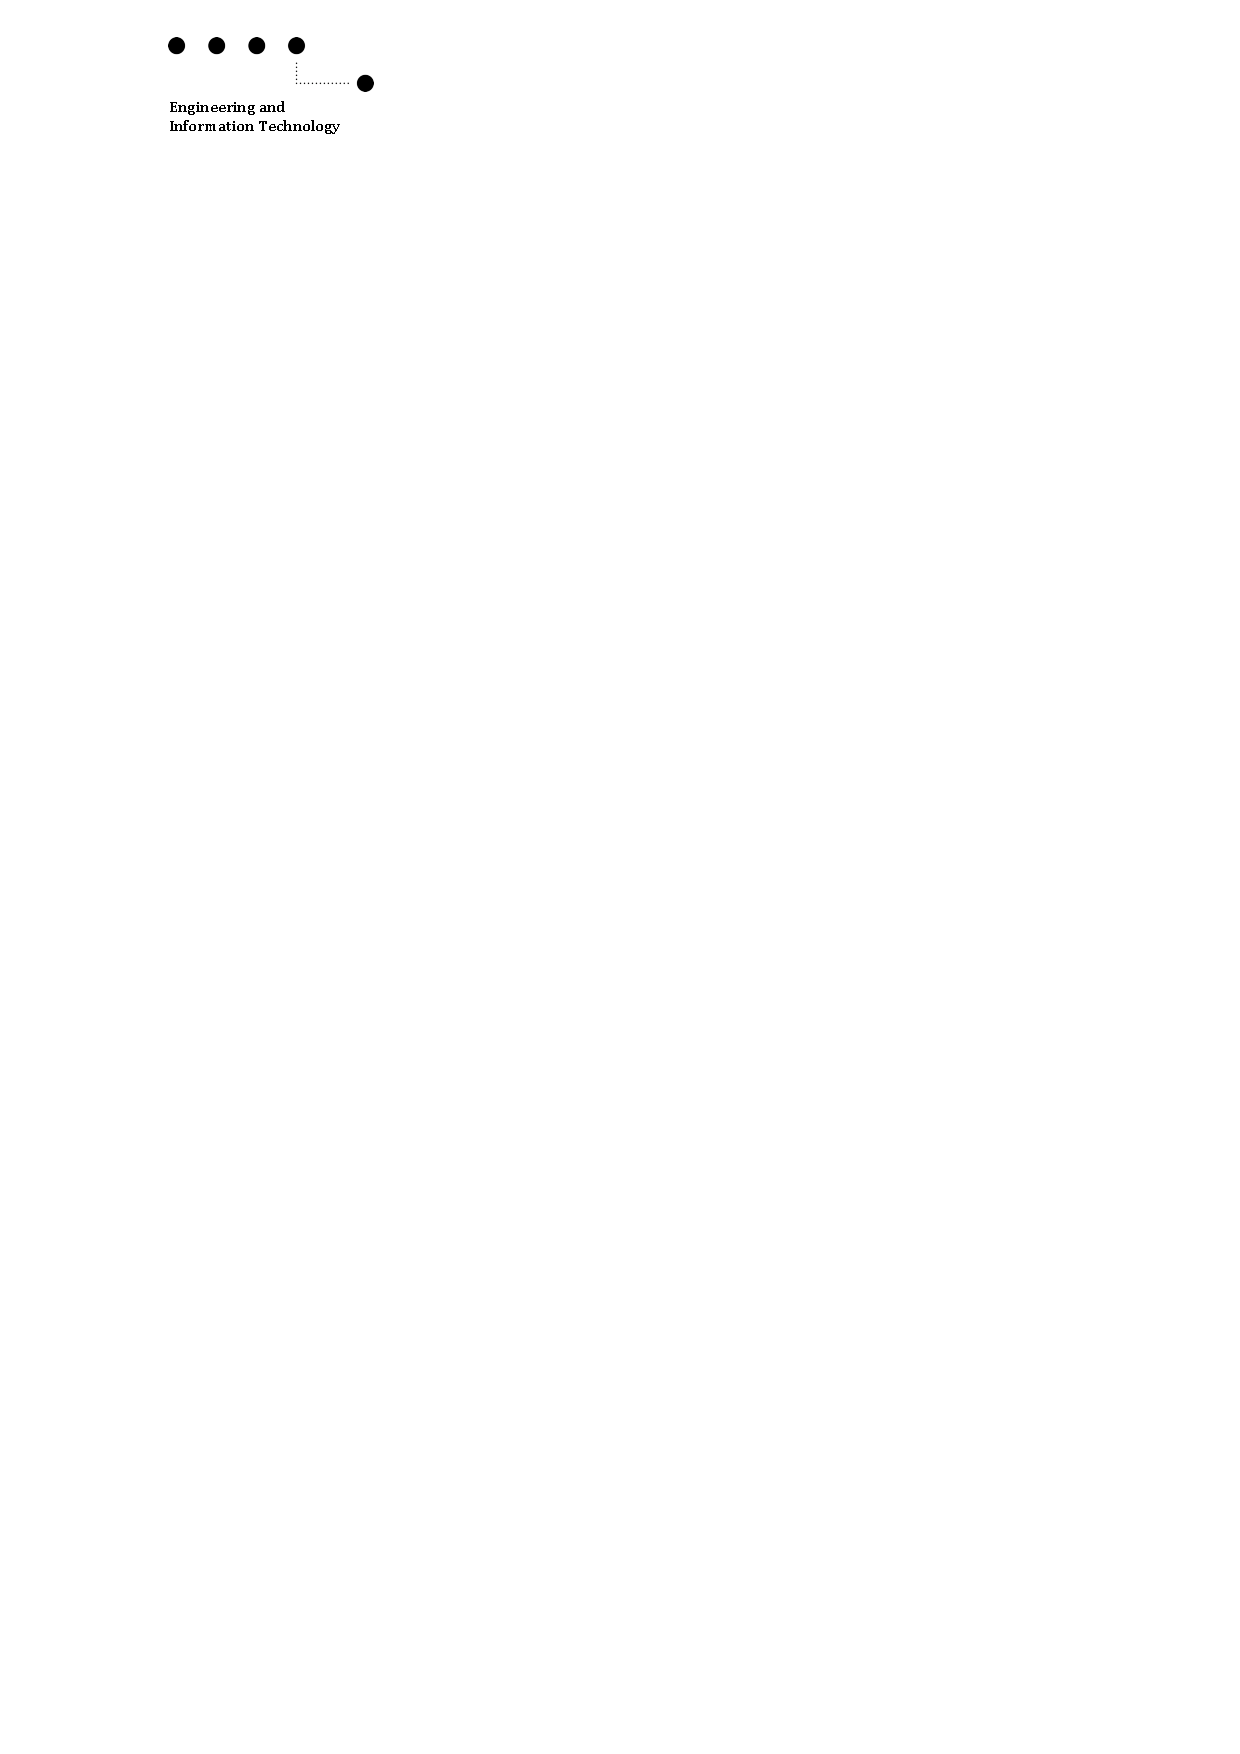
\includegraphics[height=3.5\baselineskip]{../figures/header}}
\fancyhead[RO, LE]{\leftmark}
%\fancyhead[CE]{\sectfont\bfseries \thechapter. Kapitel}
\fancyfoot[LE,RO]{\small \thepage}
\pagestyle{fancy}

 
\addtolength{\headheight}{2.2\baselineskip} 
%\addtolength{\headheight}{0.61pt}

\fancypagestyle{plain}{%
% head

\fancyhead[RE,LO]{\small \sectfont\bfseries 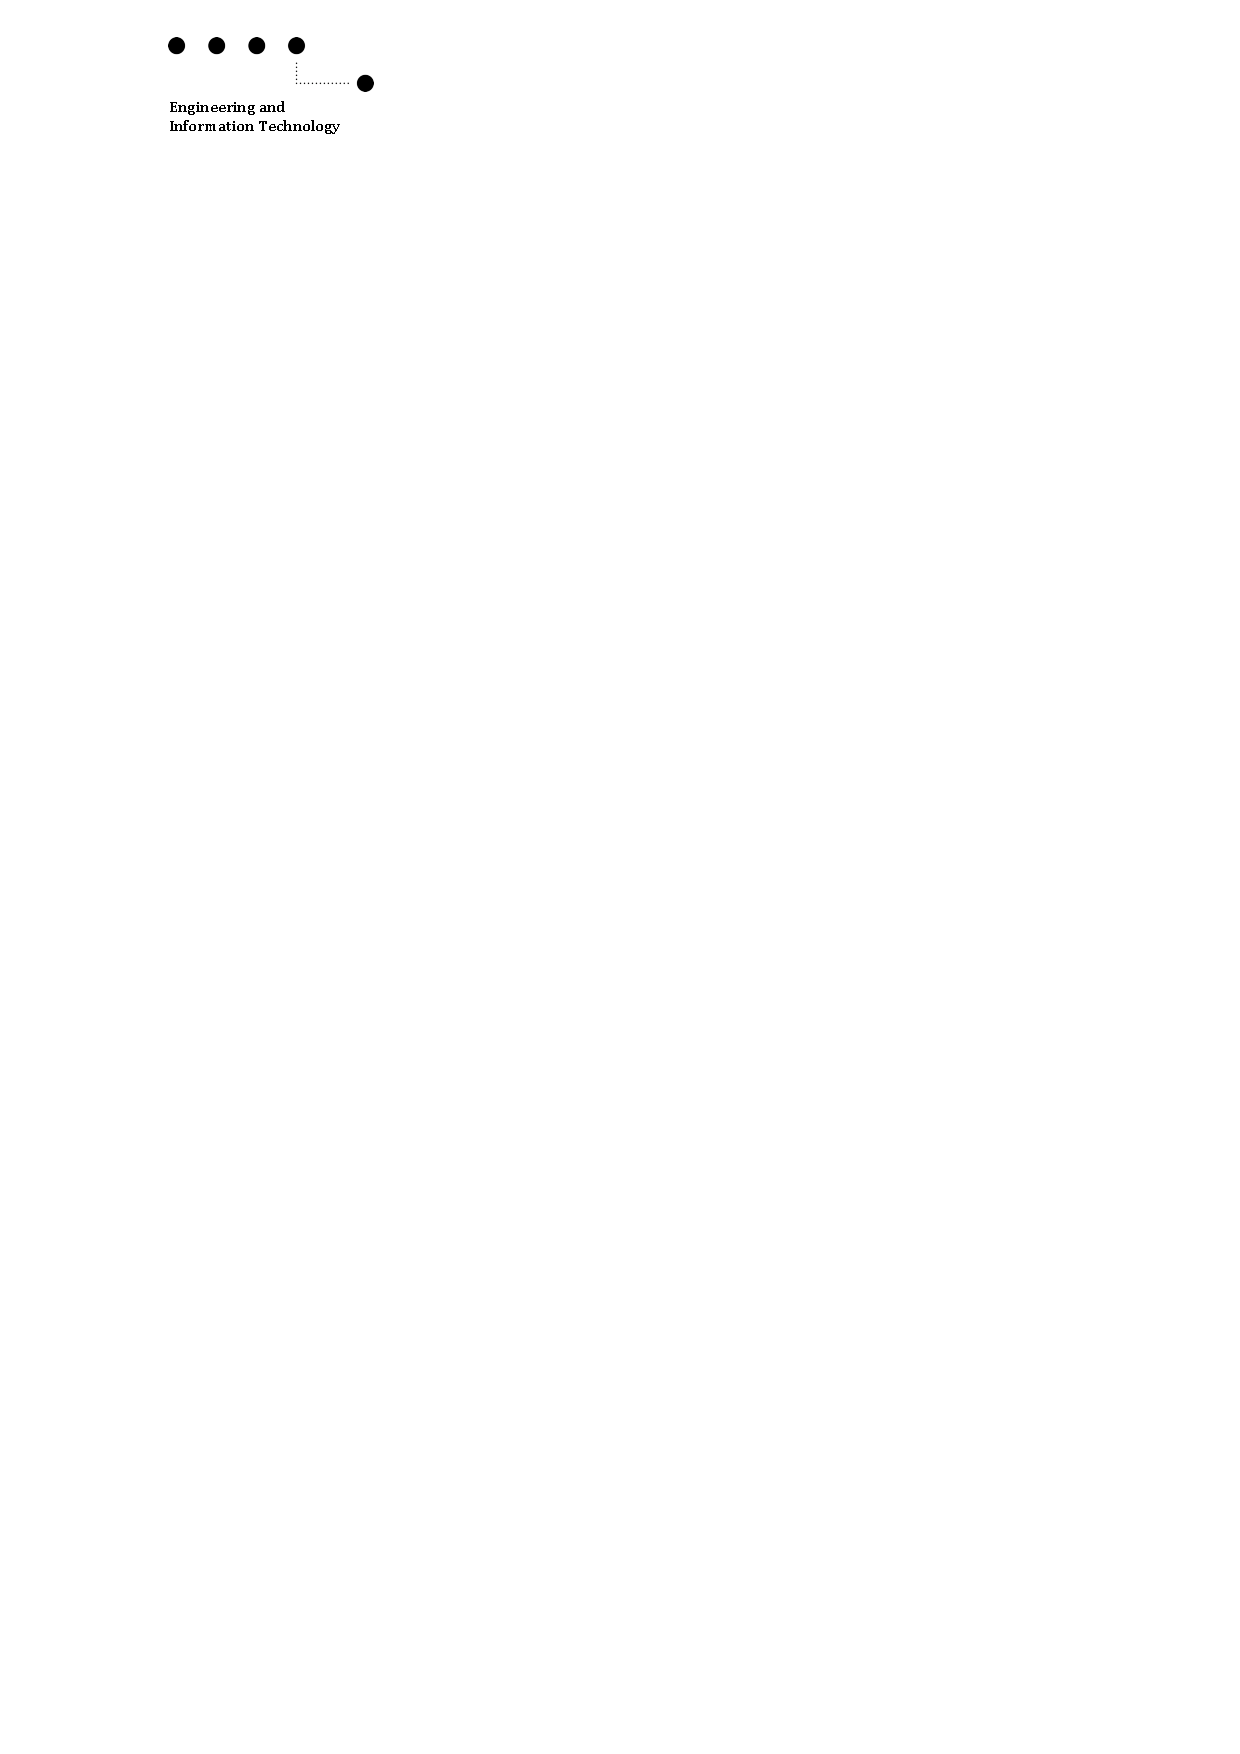
\includegraphics[height=3.5\baselineskip]{../figures/header}}
\fancyhead[RO,LE]{\leftmark}
%\fancyhead[CE]{\sectfont\bfseries \thechapter. Kapitel}
\fancyfoot[LE,RO]{\small \thepage}
\pagestyle{fancy}
}

\begin{document}
	
\begin{titlepage}
 
\begin{flushleft}

\vspace*{-2.0in}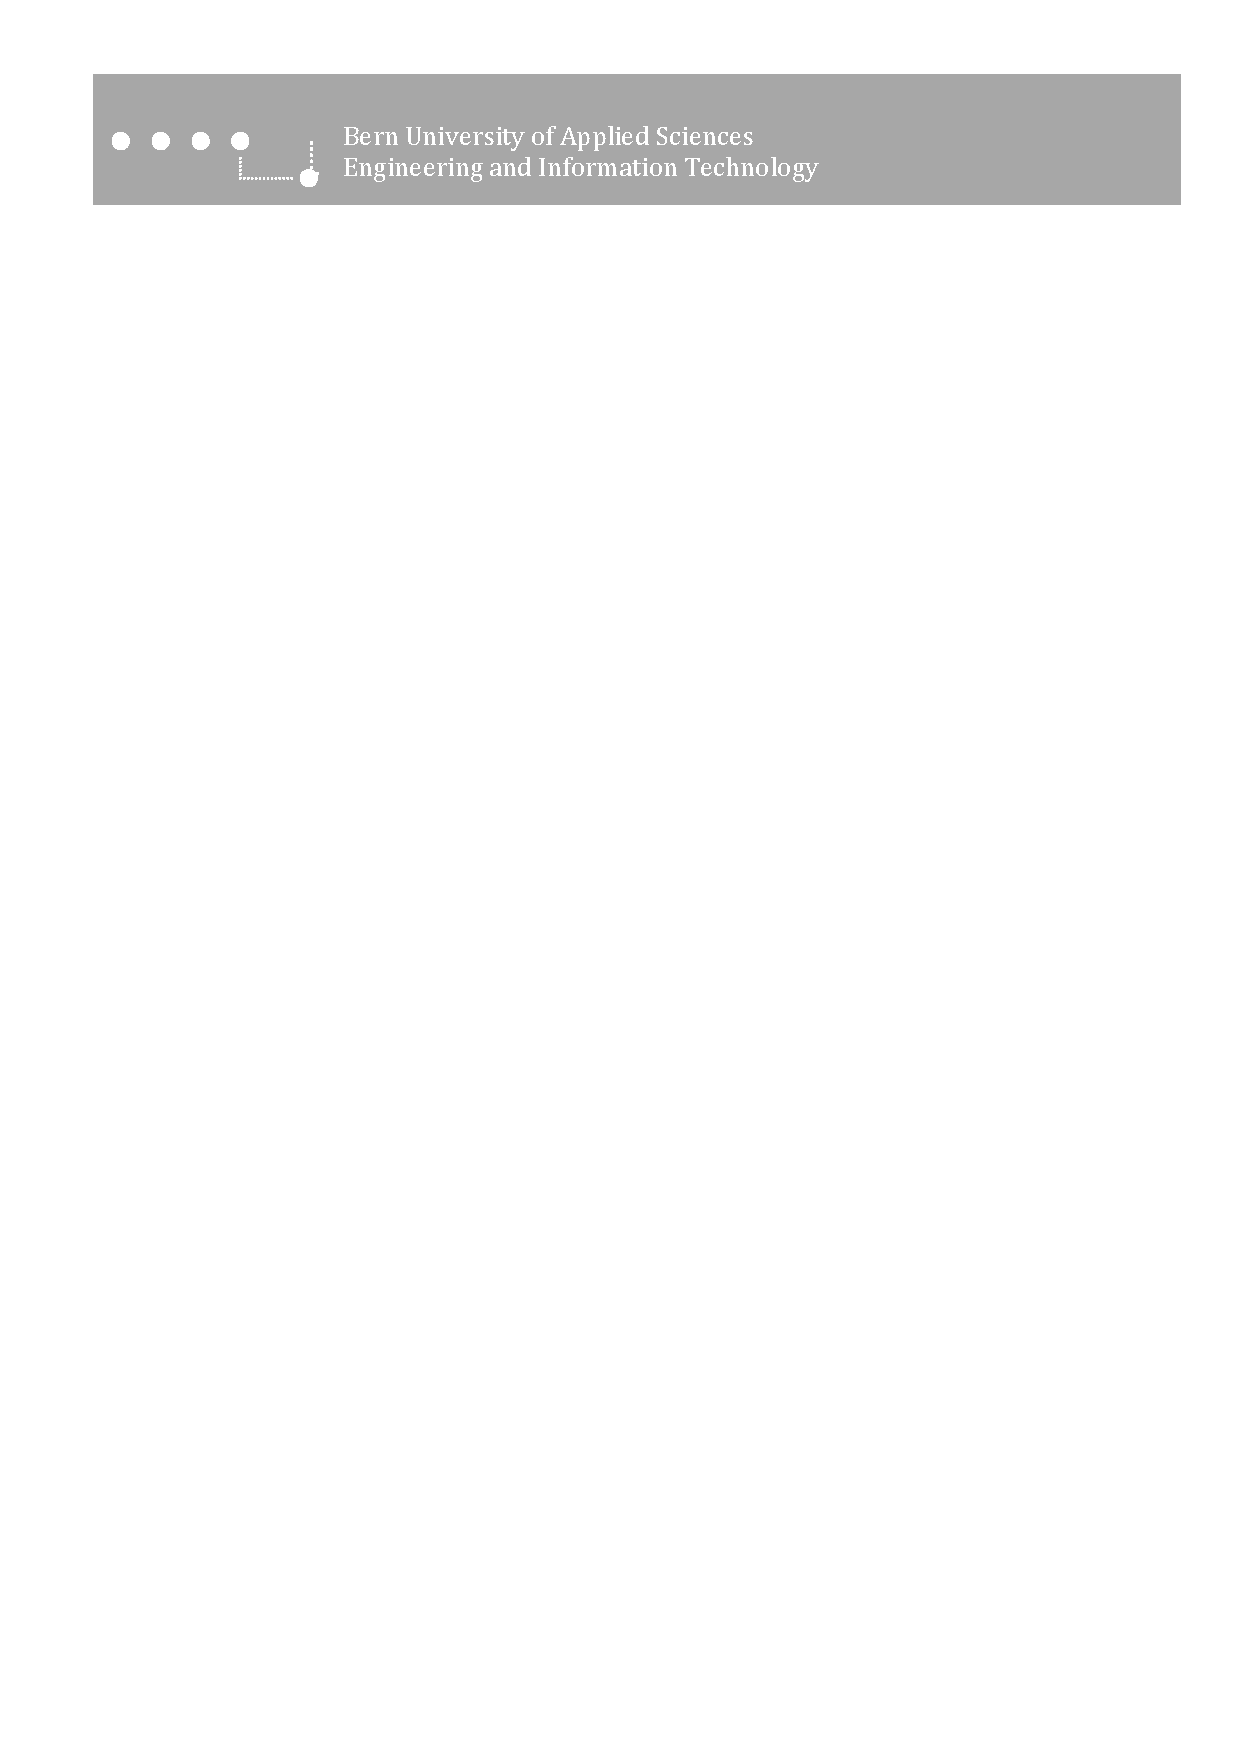
\includegraphics[scale=1.1]{../tex-include/figures/title_header}

\vspace*{2in}

\begin{tabular}{p{5cm}p{8cm}}
\Large{} & \Large{} \\ 
\end{tabular}

\vspace{1.8cm}
\begin{tabular}{ll}
\Huge{\bfseries CAVE Rendering Framework}\\[0.3cm]
\huge{Technical Report}\\[1.8cm]
\end{tabular}

\begin{tabular}{p{5cm}p{8cm}}
\Large{Division} & \Large{CPVR}\\[0.2cm]
\Large{Authors} & \Large{Brigitte Hulliger}\\[0.2cm]
& \Large{Jonas Walti}\\[0.2cm]
& \Large{Stefan Broder}\\[0.2cm]
\Large{Supervisors} & \Large{Prof. U. K\"unzler} \\[0.2cm]
& \Large{Michael Luggen }\\[0.2cm]
& \\
\Large{Version} & \Large{1.0} \\
\end{tabular} 

 \end{flushleft}
\end{titlepage}

\pagebreak
%\Large{\bfseries History}
\begin{table}
	\centering
	\begin{tabular}{|p{0.15\textwidth}|p{0.1\textwidth}|p{0.2\textwidth}|p{0.4\textwidth}|}
		\hline
		\bfseries Date & \bfseries Version & \bfseries Name & \bfseries Comment \\
		\hline
		\hline 05.06.2009 & 0.8 & all & First draft for expert H. van der Kleij \\
		\hline 09.06.2009 & 0.9 & all & Draft for Supervisors \\
		\hline 12.06.2009 & 1.0 & all & Last corrections for delivery \\
		\hline
	\end{tabular}
	\caption{History}
\end{table}
\pagebreak

\pagenumbering{roman}

\newacronym{bfhti}{BFH-TI}{Berner Fachhochschule - Technik und Informatik}
\newacronym{cpvr}{CPVR}{Computer Perception \& Virtual Reality}
\newacronym{cave}{CAVE}{Cave Automatic Virtual Environment}
\newacronym{vr}{VR}{Virtual Reality}
\newacronym{osg}{OSG}{OpenSceneGraph}
\newacronym{crf}{CRF}{CAVE Rendering Framework}
\newacronym{vrml}{VRML}{Virtual Reality Modeling Language}
\newacronym{x3d}{X3D}{}
\newacronym{opengl}{OpenGL}{Open Graphics Library}
\newacronym{glsl}{GLSL}{GL Shading Language}
\newacronym{api}{API}{Application Programming Interface}
\newacronym{ogre}{OGRE}{Object-Oriented Graphics Rendering Engine}
\newacronym{bof}{BOF}{Birds-Of-a-Feather}
\newacronym{cpu}{CPU}{central processing unit}
\newacronym{gpu}{GPU}{graphics processing unit}
\newacronym{fps}{fps}{framerate per second}
\newacronym{ascii}{ASCII}{American Standard Code for Information Interchange}
\newacronym{ssh}{SSH}{Secure Shell}
\newacronym{oo}{OO}{Object Oriented}
\newacronym{lgpl}{LGPL}{GNU Lesser General Public License}


% Inhaltsverzeichnis
\tableofcontents

% Abbildungsverzeichnis
\listoffigures

% Tabellenverzeichnis
\listoftables

% Listings 
\lstlistoflistings

\newpage
\pagenumbering{arabic}

% Abstract
% Abstract - hullb2
\begin{abstract}
	There are numerous parallel rendering frameworks and libraries applicable in visualisation systems. A relatively new approach is provided by the Equalizer API which, compared to Chromium for example, runs an application itself in parallel instead of only the generated OpenGL stream. Unfortunately, Equalizer requires knowledge about parallel rendering and synchronisation in order to get a running application. 
	
	The goal of this project was to find a solution that allows both the flexible parallel rendering of an application with Equalizer and the unlimited development of OpenGL applications without any knowledge of the Equalizer API. \gls{osg} is a high performance 3D graphics toolkit that allows the development of such feature-rich OpenGL applications and therefore provides a solution for the second requirement.
	
	The \gls{crf} provides all functionality needed to render \gls{osg} applications with Equalizer without further knowledge about parallel rendering or Equalizer. It is compatible with most Equalizer configurations and supports most of the \gls{osg} features. The purpose of the \gls{crf} is a running setup for a four sided \gls{cave} used at the \gls{bfhti}, but it is possible to use it in any visualisation system configurable with Equalizer.

\end{abstract}

% How To Read this Document - Brods1
%% How to read this document - brods1

\chapter{How to read this documents}

\subsection*{Introduction}
Our project target for the bachelor thesis was to build a framework which allows to render scenes on multiple resources. Consequently, this requirement led to Equalizer. Moreover, it was demanded to build the \gls{crf} on a common scene graph library like \gls{osg}. We soon found synergies with some other students of the University of Siegen who were already working on a similar task. As a matter of fact, they shared their achievements which helped us to get started with the \gls{crf}. Later on, we found out that that not just we, but a growing amount of other Equalizer users would be interested in an integration of \gls{osg} in Equalizer. For that reason we separated project specific documentation, e. g. the project management, from purely framework concerning documentation. Our intention is to share the latter with the Equalizer community. Hence, other users can use the \gls{crf} or even continue development. Because Equalizer users are spread all over the world, we wrote the documentation in English rather than German.

For that reason, keep in mind that the structure of this document differs from an ordinary bachelor thesis report. It is split up into four documents which can be read and distributed independently. In the following, we provide a short explanation how you should read these reports and what target group we had in mind for each document.\\
\\
We provide the following documents:
\begin{itemize}
	\item Technical Report
	\item Thesis Report
	\item User Manual
	\item Functional Specification
\end{itemize}

\section*{Thesis Report}

\subsection*{What it is}
This document focuses on our bachelor thesis. It shows how we approached our project goals, what we have done and what still needs to be done. It delivers an impression of what technologies we used and how we have chosen them. 

\subsection*{Who should read it}
This document is basically meant to be read by our supervisors Prof. U. K\"unzler and M. Luggen, and our expert H. van der Kleij.

\section*{Technical Report}

\subsection*{What it is}
The technical report describes our achievements concerning the integration of \gls{osg} into Equalizer. It contains a detailed description on the implementation and advises other programmers how to make use of it. As well it provides information on the Equalizer setup that we have worked out.

\subsection*{Who should read it}
As mentioned, there is a growing community of Equalizer users who want to take advantage of \gls{osg}. To enable interested parties to use our framework, we want to share this document as technical reference. On this account, we kept the focus in this part on the technical facts rather than organisational information or the progress during the project.

\section*{Developer Manual}

\subsection*{What it is}
On the one hand, the user manual shows \gls{cave} specific information and advices which we gathered during the bachelor thesis. The document provides a well documented guide on how to set up the required environment for our framework.

On the other hand, we want to introduce a simple \gls{osg} demo application which uses the \gls{crf}. Especially, we want to point out how to use the interface to our framework.

\subsection*{Who should read it}
The developer manual is basically meant for the \gls{bfhti} \gls{cpvr} research group or anybody interested in \gls{crf} framework.

\section*{Functional Specification}

\subsection*{What it is}
In the functional specification we specified the initial environment and evaluated the technologies we want to use. Moreover, we created use cases and defined the requirements concerning the \gls{crf}. This document helped to set limits for our bachelor thesis.

\subsection*{Who should read it}
The functional specification is given for the sake of completeness. We refer to it in the thesis report.


% Introduction - hullb2
% ==========================================
% Thesis Report - Introduction ( brods1 )
% ==========================================

\chapter{Introduction}
Over the past sixteen weeks we worked on a project within the scope of our bachelor thesis. The thesis report shows the reader what we made when we began and how we organised ourselves. Furthermore, we bring up what preparation work needed to be done, how we advanced during the project and how we tested our results. Finally, we point out unachieved goals and summarise an outlook on what could be done in the future.


% Evaluation - hullb2
% ==========================================
% Technical Report - Evaluation ( hullb2 )
% ==========================================
\chapter{Evaluation}
\label{sec:evaluation}
Due to the fact that the use of Equalizer was required for the project, the only technologies that needed to be evaluated were the two scene graph frameworks \gls{osg} and \gls{ogre}. 

A scene graph is a collection of nodes in a tree structure where a node may have many children. It arranges the logical and spatial representation of a graphical scene. The advantage of such a representation lies in the fact that an operation applied to a node in the tree automatically propagates its effect to all its children. In a graphical context this is very useful, for example, for transformations.
Scene graph technologies that were considered to be useful for this project are \gls{osg} and \gls{ogre}. Both are described below with the focus on differences rather than similarities.

% OpenSceneGraph ===========================
\section{OSG}
\gls{osg} \cite{website:osgWeb} is a cross-platform, open source and legacy-free scene graph \gls{api}. It is based upon the concept of a scene graph providing an object-oriented framework completely written in Standard C++ on top of \gls{opengl}. Therefore, a developer does not have to be concerned about optimising low-level graphics calls.

\subsection{Features}
The goal of \gls{osg} is to make the benefits of a scene graph freely available to commercial as well as non-commercial users. The key strengths of \gls{osg} are performance, portability and productivity.

\begin{description}
	\item[Performance] \hfill\\ In the core scene graph, \gls{osg} supports view-frustum culling, occlusion culling, small feature culling, Level Of Detail (LOD) nodes, \gls{opengl} state sorting, vertex arrays, vertex buffer objects, \gls{opengl} Shader Language and display lists. More features can be added by installing different plugins.
	\item[Productivity] \hfill\\ \gls{osg} makes it possible to rapidly develop high-performance graphics applications by encapsulating the majority of \gls{opengl} functionality. The developer can concentrate on content and how that content is controlled rather than low-level coding.
	\item[Portability] \hfill\\ An application developed on top of \gls{osg} can easily be ported to different platforms since the core scene graph is based on Standard C++ and \gls{opengl}. Therefore, it has minimal dependency on any specific platform. Furthermore, \gls{osg} is completely independent of windowing systems.
\end{description}

\subsection{Community}
\gls{osg} has a large community including users as well as developers. The operational area of \gls{osg} is very wide including many scientific areas. The community mostly communicates over mailing lists. There are different mailing lists for developers and users.

\subsection{Documentation}
It is recommended to start with the book \emph{OpenSceneGraph Quick Start Guide}\cite{osgGuide} written by Paul Martz.
Other than that \gls{osg} depends on the community for documentation. The official website of \gls{osg} is a wiki. The reason for that is that \gls{osg} wants its users and developers to be able to document their features themselves. On the one hand this is very useful since all documentation can be found on the same website. On the other hand this approach leads to a slightly unorganised website.

% OGRE =====================================
\section{OGRE - Object-Oriented Graphics Rendering Engine}
\gls{ogre} \cite{website:ogreWeb} is a 3D engine based on the scene graph concept. As \gls{osg}, it is completely written in Standard C++. The underlying libraries are Direct3D or \gls{opengl}. \gls{ogre} is available under the LGPL (GNU Lesser General Public License\footnote{\href{http://www.gnu.org/copyleft/lesser.html}{http://www.gnu.org/copyleft/lesser.html}}).

\subsection{Features}
\gls{ogre} puts emphasis on the design of the engine. The developers of \gls{ogre} pursue the strategy of well designed and well documented features instead of a high number of features, or in other words: quality over quantity.

\subsection{Community}
The community of \gls{ogre} is comparable with the one of \gls{osg}. Besides mailing lists, \gls{ogre} comes with forums and an IRC channel for communication.

\subsection{Documentation}
The approach of design-led rather than feature-led is reflected in the documentation of \gls{ogre}. Together with multiple books \gls{ogre} comes with an \gls{api} reference, a manual and a wiki.


% \gls{osg} vs. OGRE =============================
\subsection{OSG vs. OGRE}
Both of the discussed scene graph \glspl{api} were considered for integration with Equalizer. For comparison of the two technologies, it makes sense to use a decision matrix. The scale reaches from 1 to 10 where 10 is the highest value. Each point in the decision matrix can be weighted differently depending on the importance in the current project.

\begin{table}[ht]
	\centering
	\begin{tabular}{|l|c||c|c|c||c|c|c|c|}
		\multicolumn{2}{r}{ }			&	\multicolumn{3}{c}{\bfseries OSG}	&	\multicolumn{3}{c}{\bfseries OGRE} 	\\
		\hline
		Criteria		& Weight		&	Value	& Points	& \%Points		&	Value	& Points	& \%Points		\\
		\hline
		Performance I 	& 25\%			&	160fps	& 3			& 75			&	220fps	& 7			& 175			\\
		Performance II	& 25\%			&	260fps	& 7			& 175			&	220fps	& 3			& 75			\\
		Community		& 10\%			& 	++		& 4			& 40			&	+++		& 6			& 60			\\
		Similar Projects& 20\%			& 	eqOSG	& 7			& 140			&	eqOGRE	& 3			& 60			\\
		Documentation	& 10\%			&	++		& 4			& 40			&	+++		& 6			& 60			\\
		Extensions		& 10\%			&	++		& 4			& 40			&	+++		& 6			& 60			\\
		\hline
		\hline
		\bfseries Total	&\bfseries 100\%&	\multicolumn{3}{c||}{\bfseries 510}	&	\multicolumn{3}{c|}{\bfseries 490}	\\
		\hline	
	\end{tabular}
	\caption{Decision Matrix OSG - OGRE}
	\label{tab:DecisionMatrix}
\end{table}

A stress test application was used to test the performance. This application consists of a three dimensional model consisting of about one billion triangles in an empty universe. The workstation used for the tests was an Intel Pentium Quadcore with an NVIDIA graphics chip. Two different measures were made based on this setup:
\begin{description}
	\item[Performance I] 	The framerate (frames per second) when the whole model is visible.
	\item[Performance II]	The framerate when only a part of the model on the screen (by zooming into the scene until some parts of the scene are outside of the frustum).
\end{description}
The result of this test setup was that \gls{ogre} does not show any differences between the setup with the whole model on the screen and the one where only part of the model is visible. In \gls{osg} on the other hand, the framerate increases if part of the model is outside of the frustum.

\gls{ogre} wins the competition in the criteria \emph{Community} because \gls{ogre} provides more communication channels (forum, mailing list, IRC channel) than \gls{osg} and the communication seems to be better organised.

Looking for extensions both of the participants are up-to-date. There are miscellaneous 3rd party extensions that can be installed. Most of them are freely available. The most interesting extensions for this evaluation were physics and haptics plugins. Both are available for \gls{osg} and \gls{ogre}.

Considering all these criteria, \gls{osg} wins the competition as one can see from the result of the decision matrix above. Although, the decision is quite marginal and is mostly based on the fact that there is a project called \emph{eqOSG}, which is currently under development at the University of Siegen (Germany) and that \gls{osg} has a large community in science.


% Equalizer - hullb2
\subsection{Equalizer}
Equalizer ist ein Framework zur Erstellung von parallelen, OpenGL-basierten Applikationen. Es erm"oglicht, Applikationen auf mehreren Grafikkarten, Prozessoren und Computern zu renderen und somit die Performance zu verbessern. 
Eine auf Equalizer basierende Applikation kann unver"andert aus verschiedenen Visualisierungssystemen ( Workstations, Cluster, Virtual Reality Installationen, etc) gestartet werden.

\paragraph{}
Das Equalizer-Projekt ist richtungsweisend und einzigartig was paralleles Rendering anbelangt. Initiator und Hauptentwickler Stefan Eilemann ist der BFH-TI nicht unbekannt und mit ihm wurden bereits Kontakte gekn"upft. Da es nichts vergleichbares gibt und gute Kontakte bestehen, ist die Verwendung von Equalizer vorgegeben. Ausserdem wird Equalizer rege genutzt und stetig weiterentwickelt. 

\subsubsection{Equalizer im CAVE}
Equalizer unterst"utzt sowohl aktives wie auch passives Stereo Rendering. Dabei gibt es die M"oglichkeit, dass jede Stereo View auf einer separaten CPU und Grafikkarte gerenderet werden kann. 

\begin{figure}[ht]
\begin{center}
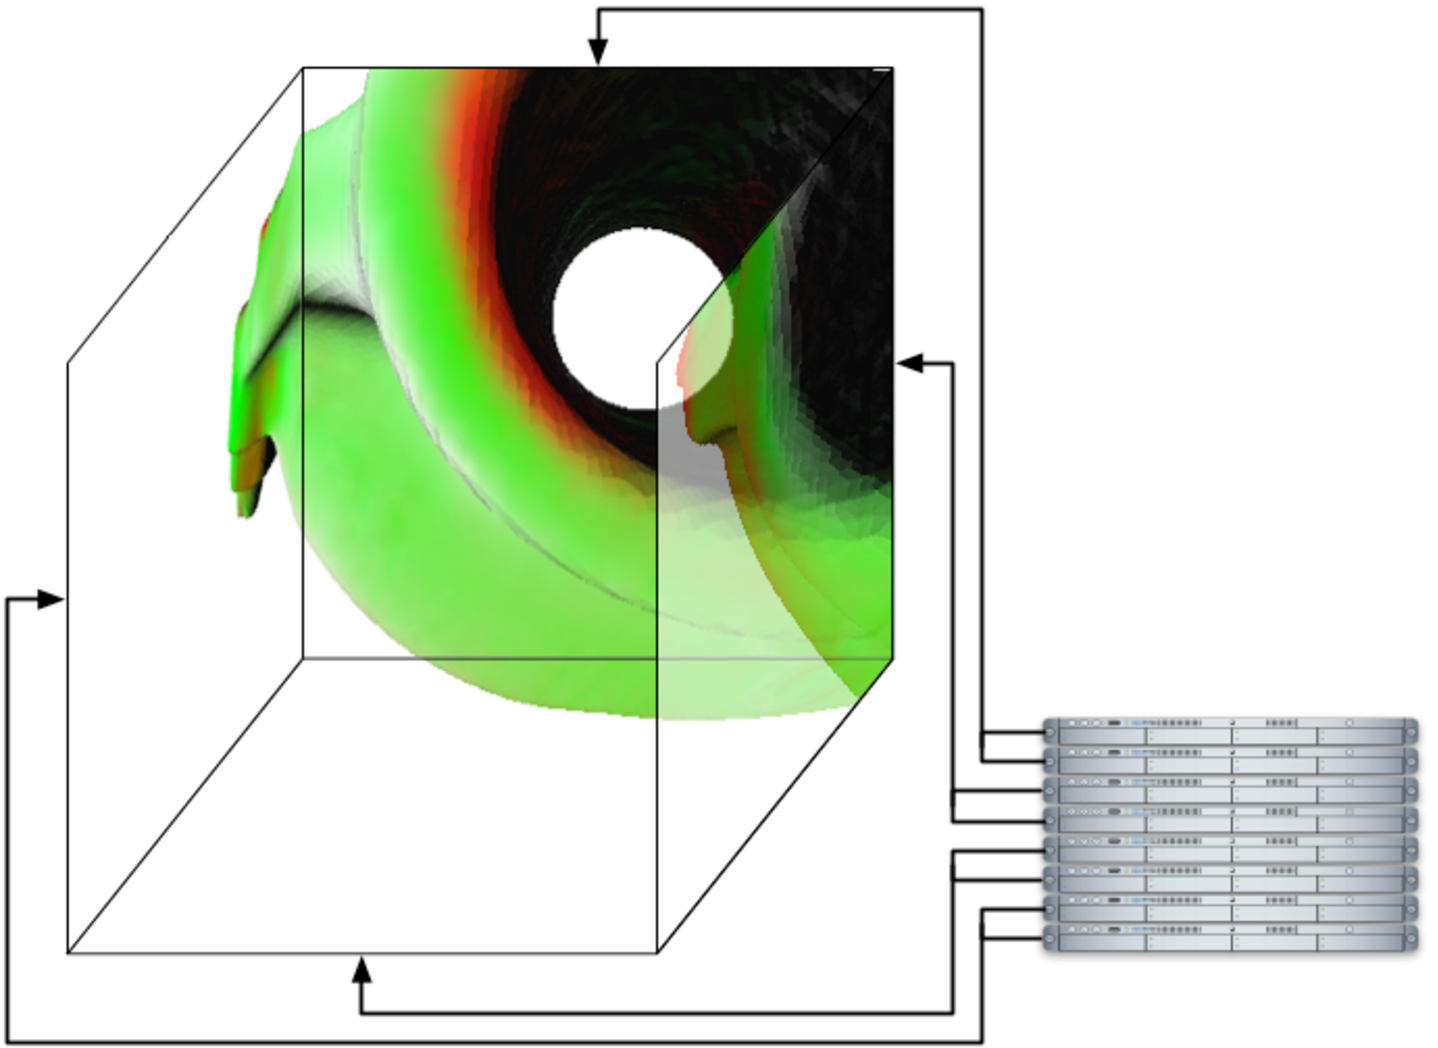
\includegraphics[scale=0.3]{../figures/equalizer_cave}
\end{center}
\caption{Equalizer im CAVE (Quelle: [5])}
\end{figure} 

\begin{figure}[ht]
\begin{center}
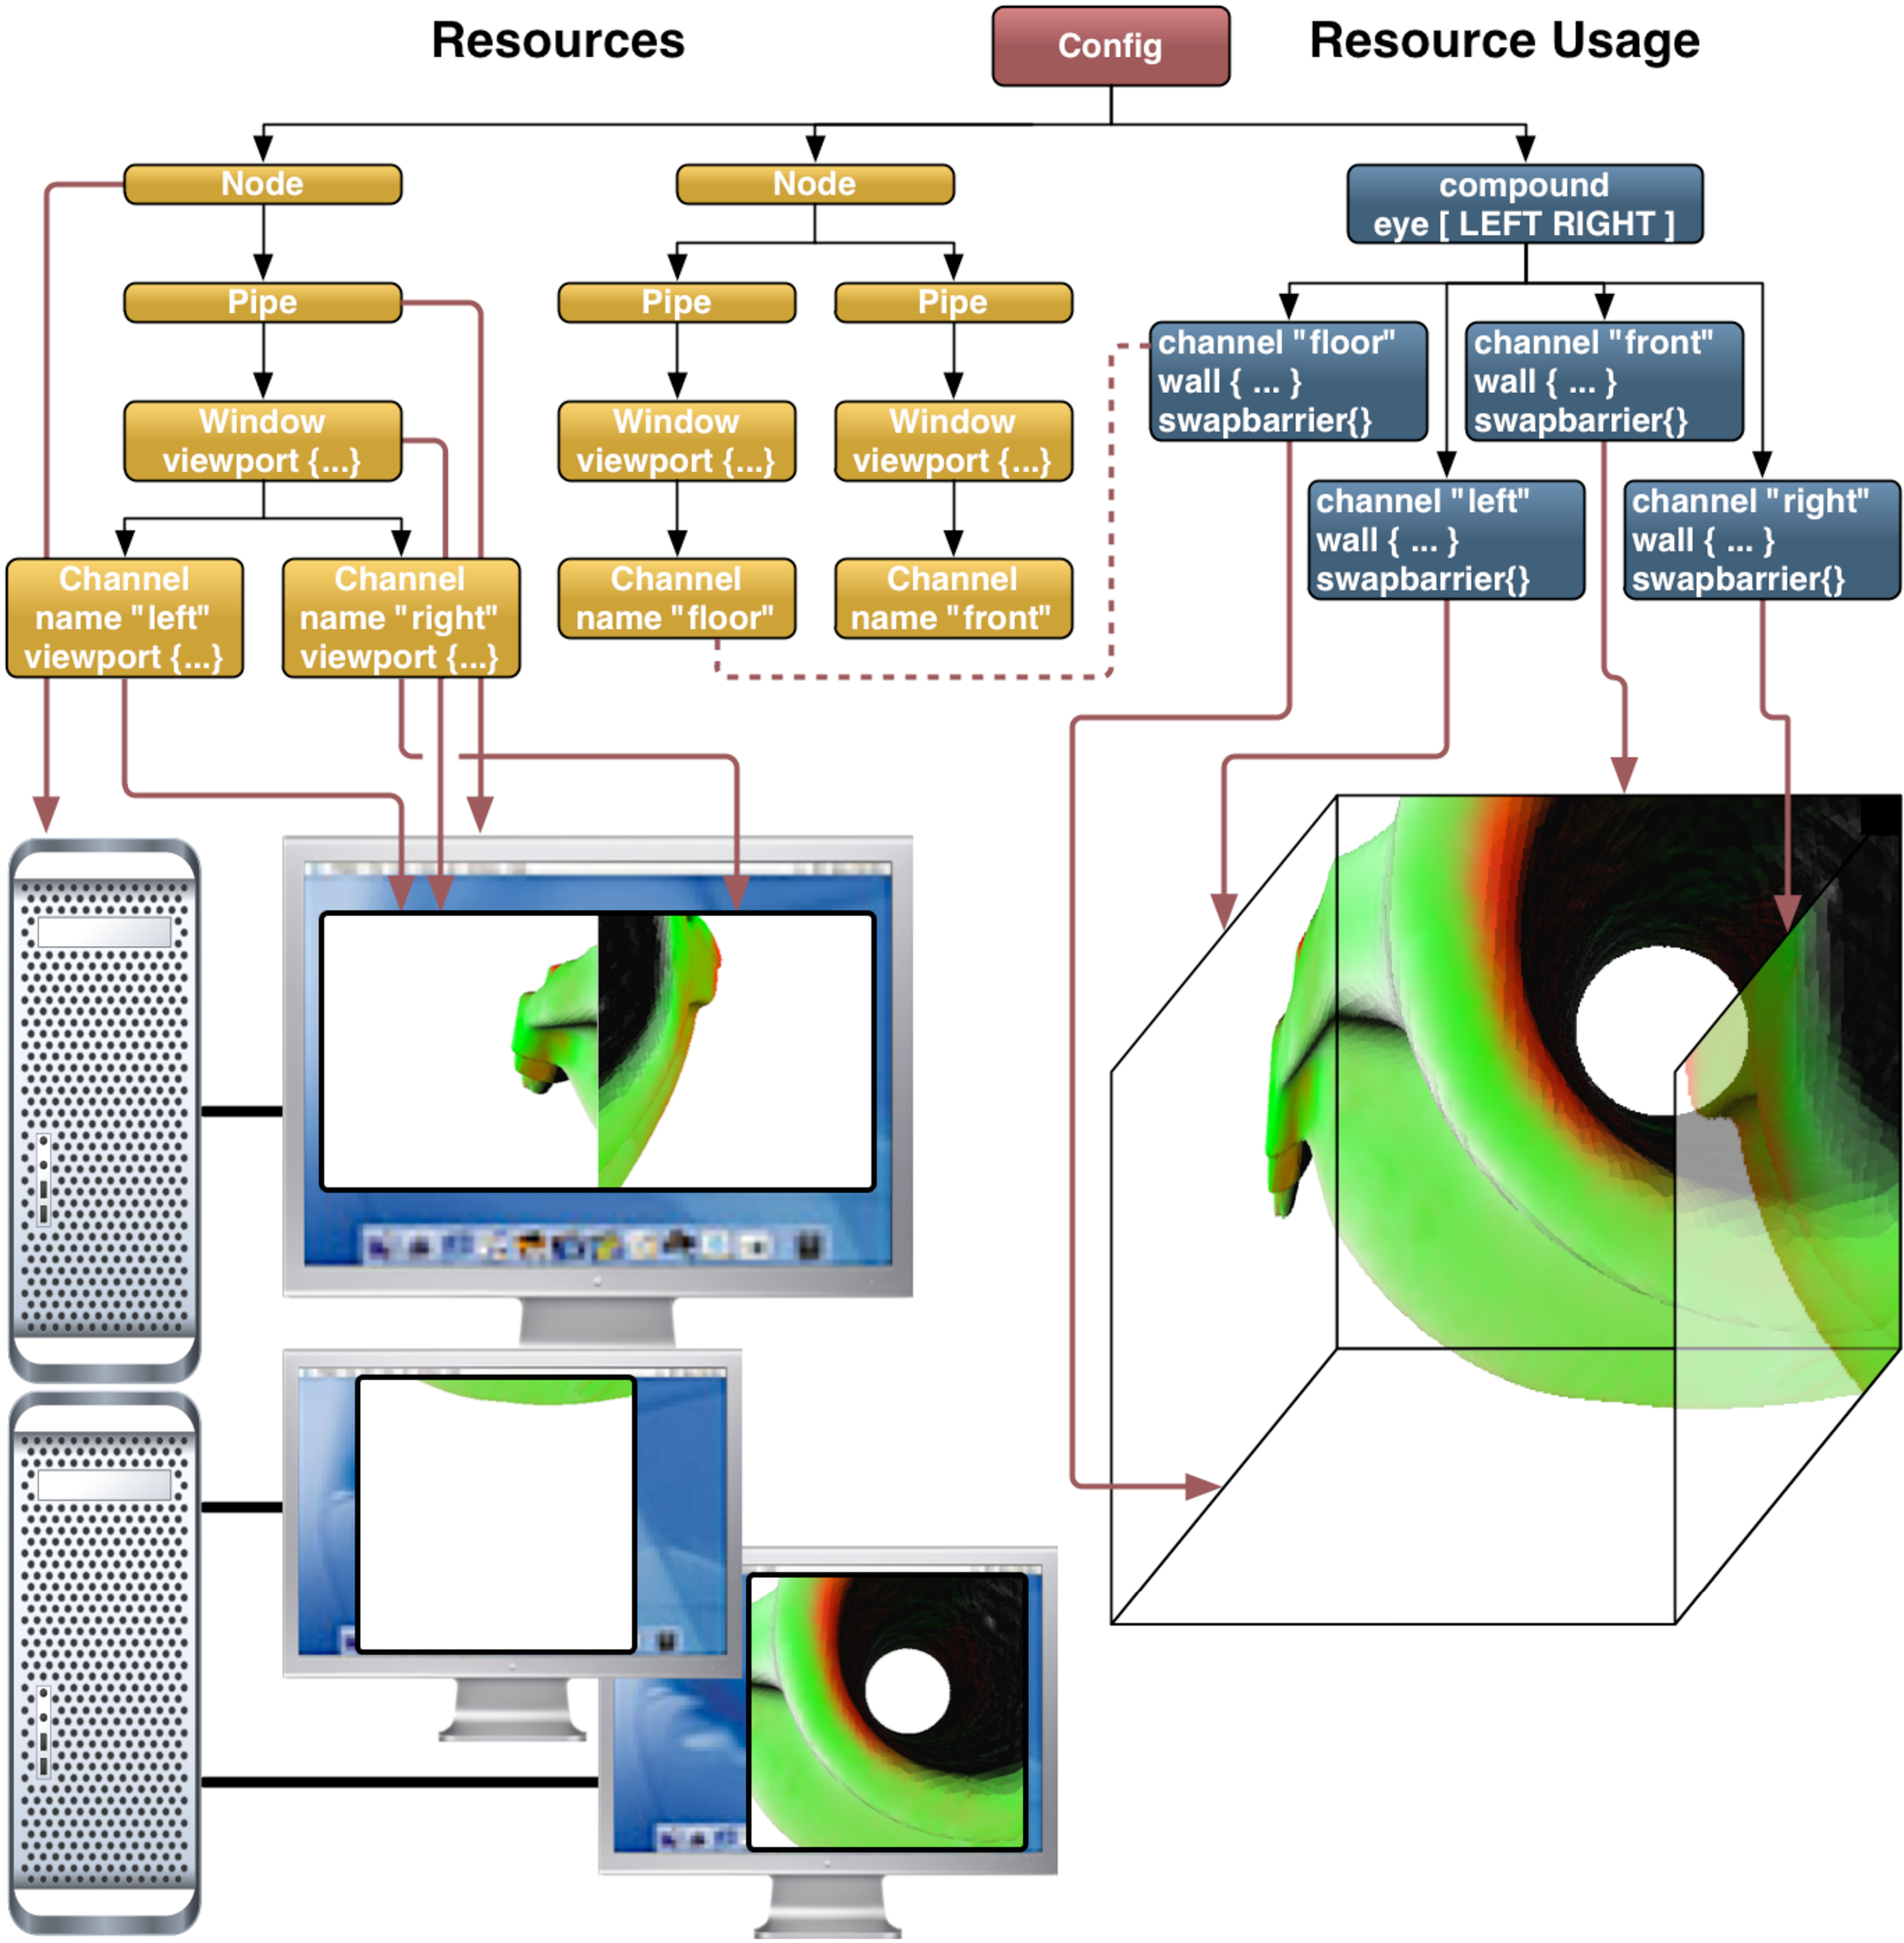
\includegraphics[scale=0.2]{../figures/equalizer_resources}
\end{center}
\caption{Equalizer im CAVE - Beispiel Konfiguration (Quelle: [1, Seite 10]}
\label{eq_ex_config}
\end{figure}


% Framework - waltj3
% ==========================================
% Technical Report - Framework ( waltj3 )
% ==========================================
\chapter{CAVE Rendering Framework}

\section{Idea}

The main goal of this framework is to provide a simple tool library to render \gls{osg} applications with Equalizer. \gls{osg} developers do not need a lot of knowledge of Equalizer. The \gls{crf} offers simple methods to pass the \gls{osg} scene graph to Equalizer for basic \gls{osg} applications with static scene graphs. Furthermore, it provides additional tools to handle more complex \gls{osg} applications with user input and highly dynamic scenes.

Nevertheless, the final application is compatible with most Equalizer configurations and supports most \gls{osg} features. For further information about this, have a look at the section \nameref{sec:crfLimitations} or \nameref{chap:Testing}.

\section{Design}
\subsection{Design Techniques}
The \gls{crf} abstracts the more complex Equalizer framework. Similar, to many common frameworks, the \emph{Hollywood Principle}\footnote{\emph{The Hollywood Principle} is a well known paradigm in software engineering. \emph{Don't call us, we call you}, meaning the implemented functions are called by the framework than the developer.} plays a major role in the Equalizer framework and therefore also in our \gls{crf}. To provide an easy interface for simple \gls{osg} applications, we implemented the \texttt{crfStarter} class in a facade pattern\footnote{The facade pattern is a software engineering design pattern commonly used in \gls{oo} programming. The name is in analogy to an architectural facade. A facade is an object that provides a simplified interface to a larger body of code, such as a class library.} manor. This class provides easily understandable functions, which pass the \gls{osg} scene graph to the framework and run it with Equalizer.

\section{Namespaces}
\begin{description}
	\item[namespace \texttt{eq}] \hfill\\The low-level standard Equalizer namespace. When using the basic \gls{crf} features, one should not have to care about this namespace.
	\item[namespace \texttt{osg, osgViewer, osgGA, $\dots$}] \hfill\\Naturally, the \gls{crf} uses some of the \gls{osg} classes.
	\item[namespace \texttt{eqOsg}] \hfill\\The basic implementation for rendering \gls{osg} scene graphs with Equalizer. This namespace contains the implementations of all the must-have Equalizer classes to build a complete Equalizer application with a scene graph. Moreover, some basic features, like a camera control and the specialised \texttt{EqViewer}, which inherits from the standard \texttt{osgViewer}, are implemented here.
	\item[namespace \texttt{crf}] \hfill\\This namespace provides classes to abstract the \texttt{eqOSG} Equalizer application. Classes like \texttt{crfPipe}, \texttt{crfChannel} and the facade class \texttt{crfStarter} provide easily usable functions to run an \gls{osg} scene graph with Equalizer.
\end{description} 

\begin{figure}[H]
	\centering
		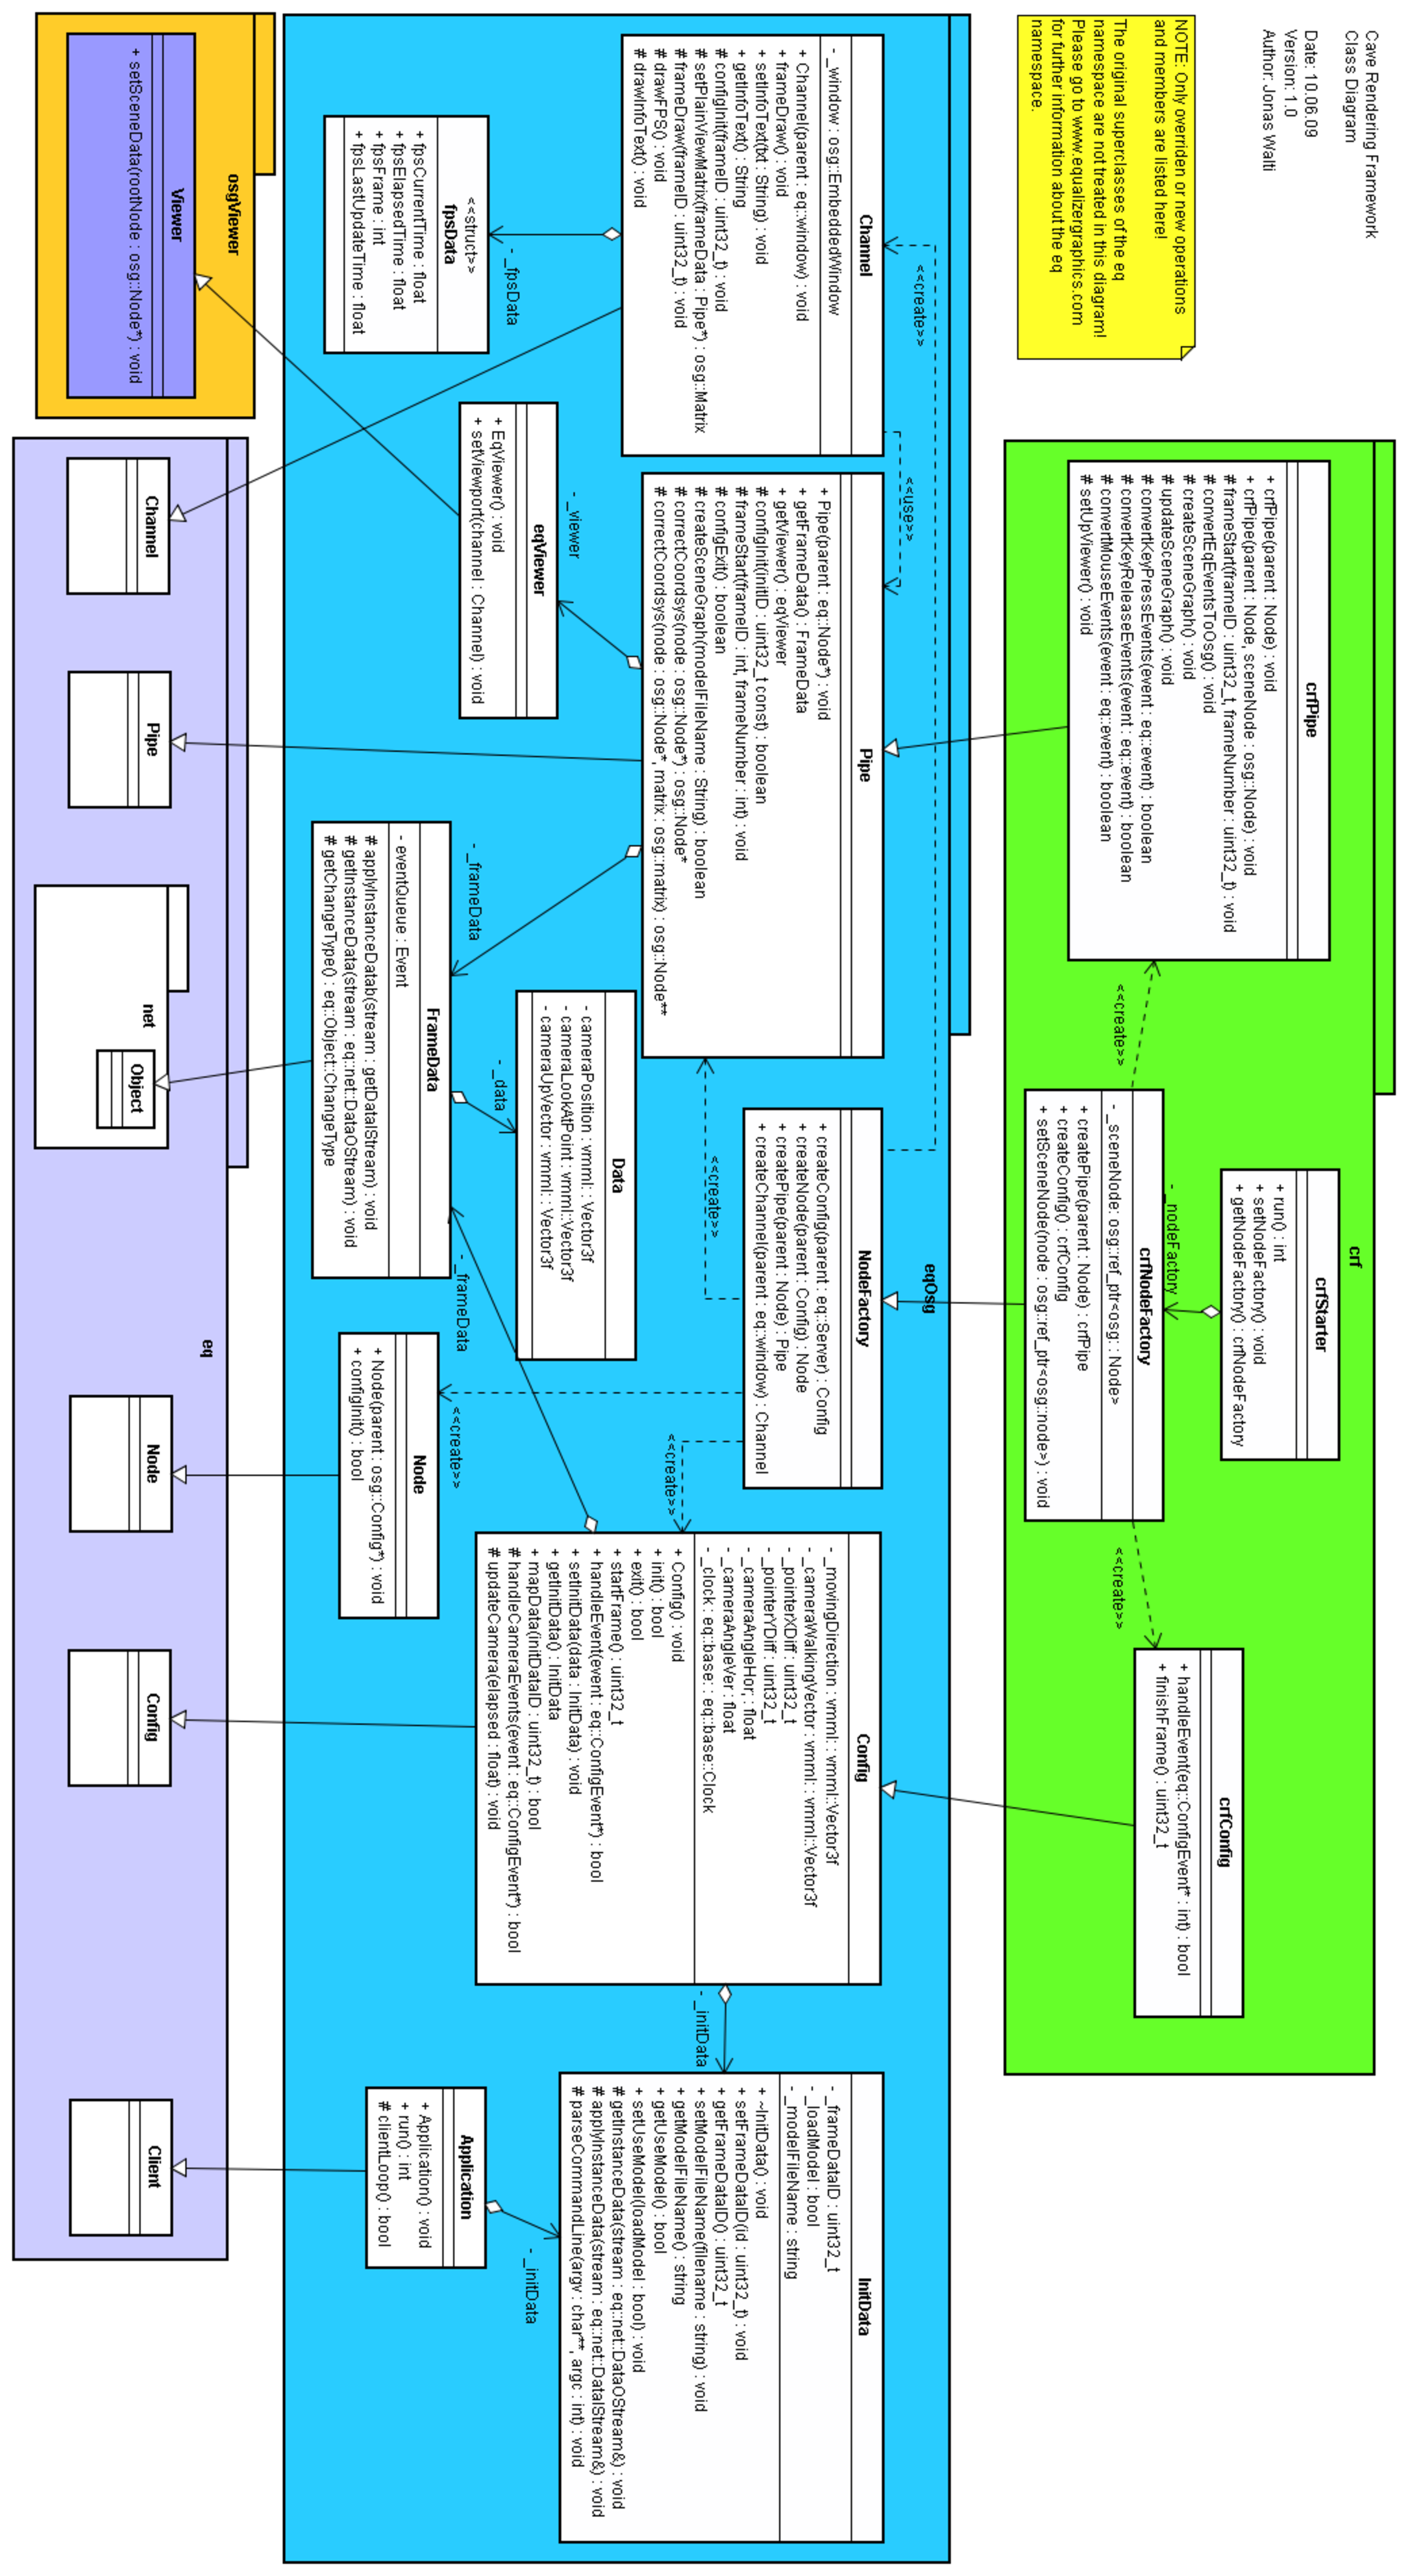
\includegraphics[width=0.850\textwidth,angle=180]{../figures/crf_class_diagram_complete_01}
	\caption{The complete class diagram with all three namespaces}
	\label{fig:crf_class_diagram_complete_01}
\end{figure}

\section{Implementation}
\subsection{About this section}
The information provided in this section cares about technical implementation facts. This may help a framework user to fix errors.

IMPORTANT: This part of the documentation requires knowledge of Equalizer. Please consult the previous Equalizer section or the Equalizer Programming Guide \cite{eqPG} for further information.

\subsection{Overview}
Equalizer applications in general are realised by subclassing existing classes of the \texttt{eq} namespace. A good example is the \texttt{eqPly} application, shipped with Equalizer. This example makes use of much Equalizer functionality. However, it has nothing to do with \gls{osg}.

In the \gls{crf} implementation, every pipe holds a complete \texttt{eqOsg::EqViewer}, which inherits from \texttt{osgViewer::Viewer}. Hence, every pipe holds a complete and fully independent scene graph. This is very important because this can force synchronisation problems and therefore errors in multipipe and/or multinode Equalizer configurations.

The only communication between this different scene graphs is realised with the \texttt{FrameData} class. \texttt{FrameData} inherits from the \texttt{eq::net::Object} class. This object has to be converted to a stream in order to pass it over the network in multinode configurations. In the basic \texttt{eqOsg::FrameData} class, several members are present to describe the cameras position, up-vector, viewing direction and current state. 

\subsection{\texttt{eqOsg} namepsace classes}
\label{sec:Overview}\hfill\\
Classes in the \texttt{eqOSG} namespace provide a basic Equalizer application with an \gls{osg} viewer. All needed functionality to render an \gls{osg} scene graph with Equalizer are implemented here.

\begin{description}
	\item [class \texttt{EqViewer}]\hfill\\
		The \texttt{EqViewer} class inherits from the original \texttt{osgViewer::viewer} and provides a viewer, which is used to render an \gls{osg} scene with Equalizer, because the default \texttt{osgViewer} does not work. Listing \ref{lst:eqViewer} shows the important line of code in the constructor.

	\begin{lstlisting}[caption={Constructor of the \texttt{EqViewer}},label={lst:eqViewer}]
	EqViewer::EqViewer()
	{
		//makes the viewer single threaded
		setThreadingModel(osgViewer::Viewer::SingleThreaded);

	}
	\end{lstlisting}
	Because a default \gls{osg} viewer does not support the multithreaded mode if configured as embedded window (what is needed here, because Equalizer creates the windows), the threading model is set to single. The newly added function \texttt{setViewport(eq::channel channel)} sets the frustum and the viewport of the camera, depending on the Equalizer configuration and the passed Equalizer channel.
	\item[class \texttt{Config}]\hfill\\
		As in a common Equalizer applications, \texttt{osgEq::Config} represents the current configuration of the application. It also updates the frame data class when necessary. Additionally, the \texttt{eqOsg::Config} class calculates the position and viewing direction of the camera. This happens by receiving mouse and keyboard events in \texttt{Config::handleEvents()}. Afterwards, calculating the new cameras properties in \texttt{Config::updateCamera()}. Finally, the new camera properties are updated in the frame data. \\ The rest is similar to the eqPly example.
	\item[class \texttt{FrameData}]\hfill\\
		The \texttt{FrameData} class is a container for values which can be sent to every node and pipe. This is the only way to pass (updated) data to the different render clients and pipes at runtime. In the \texttt{eqOsg::FrameData} class, all information concerning the camera is stored in this object.
	\item[class \texttt{Application}]\hfill\\
		The \texttt{eqOsg::Application} class is similar to the eqPly example. This class starts and stops the application, runs the main loop by calling the \texttt{startFrame()}, and \texttt{finishFrame()} functions of the \texttt{Config} object.
	\item[class \texttt{NodeFactory}]\hfill\\
		The \texttt{eqOsg::NodeFactory} is needed to create the desired objects during the initialisation of Equalizer.
	\item [class \texttt{Node}]\hfill\\
		As in a standard Equalizer application, the node class represents a render client. This class does not contain important changes, because the \gls{crf} does not need node-specific customisations.
	\item [class \texttt{Pipe}]\hfill\\
		The class \texttt{Pipe} abstracts a physical \gls{gpu}. The derived class \texttt{eqOsg::Pipe} holds the two additional members; The \texttt{osgEq::EqViewer} \texttt{\_viewer} and the \texttt{eqOsg::FrameData} \texttt{\_frameData}. The viewer holds the complete scene graph and frame data, which is a copy of the distributed data. \texttt{eqOsg::Pipe} is a basic and lightweight implementation with an empty scene graph. The \texttt{crf::crfPipe} inherits from this class and provides additional functions to create and update the scene graph. More information about this can be found in the following sections.% (\ref{sec:...}).
	\item [class \texttt{InitData}]\hfill\\
		The \texttt{eqOsg::InitData} class is needed during the initialisation of the application. It also provides a function to parse the command line and set this initial data. Furthermore, it holds the frame data ID, so all clients can synchronise on the distributed frame data object.
	\item [class \texttt{Channel}]\hfill\\
 		In Equalizer a \texttt{Channel} represents an \gls{opengl} viewport. Hence, \texttt{eqOsg::Channel} renders the scene graph. This is done with the \texttt{frameDraw()} function. Consult \ref{sec:FrameRendering} for more information. Moreover, when the \texttt{configInit} function of the channel is called, the \texttt{EqViewer} will be configured as an embedded window. This ensures that a virtual \gls{osg} window is defined, which is widely used in given \gls{osg} classes (for example \texttt{osgViewer::StatsHandler} or \texttt{osgGA::FlightManipulator}).
\end{description}

  
\subsection{\textbf{\texttt{crf}} namepsace classes}
\hfill\\
The \texttt{crf} namespace contains more specialised classes to render \gls{osg} applications with Equalizer. The lightweight  \texttt{eqOsg} namespace provides only basic features to render an \gls{osg} scene graph. The derived classes of the \texttt{crf} namespace implement additional functionality for showing statistics, scene graph coordinate system correction and the \texttt{crfStarter} class as a facade for simple execution of the application.
\begin{description}
	\item[class \texttt{crfNodeFactory}]\hfill\\
		This class inherits from the \texttt{eqOsg::NodeFactory} and is used by the \texttt{crfStarter} class to create the desired Equalizer objects.
	\item[class \texttt{crfStarter}]\hfill\\
		The \texttt{crfStarter} is the facade class of our framework. With this class it is possible to run an Equalizer \gls{osg} application with two lines of code shown in listing \ref{lst:crfStarter}.
		
		\begin{lstlisting}[caption={\texttt{crfStarter} main method},label={lst:crfStarter}]
		#include <crf/crfStarter.h>

		//1. Create the main method, which calls the crfStart.run() 
		//method to start equalizer and stuff
		int main(int argc, char** argv) 
		{
		    //create the \gls{crf} starter
			crf::crfStarter starter;

			//run the application
			starter.run(argc,argv);
		}
		\end{lstlisting}

		In this special case, a HelloWorld application will be started because no node factory and no \gls{osg} node have been passed to the starter object. For simple scene graphs, it is possible to pass an \gls{osg} root node as third argument of the \texttt{starter.run(...)} method. For dynamic and more complex \gls{osg} applications, custom classes have to be implemented (by subclassing the desired \texttt{eqOsg} and \texttt{crf} classes) and a custom node factory has to be passed to the starter with \texttt{starter.setNodeFactory(yourCustomFactory)}.
	\item[class \texttt{crfPipe}]\hfill\\
		This class extends the \texttt{eqOsg::Pipe} with features like pushing Equalizer events to the \gls{osg} viewer, scene graph updates, scene graph rotation and more. 
\end{description}

\subsection{OSG Rendering With Equalizer}
\subsubsection{Overview}
\label{sec:Overview}
This section explains how the scene graph is rendered with Equalizer. In the \emph{eqPly} or the \emph{eqHello} example of Equalizer, there is native OpenGL code in the \texttt{Channel::frameDraw()} function. But in the \gls{crf}, the OpenGL commands come from the \gls{osg} viewer's camera and have to be rendered considering every channel's viewing matrix. 

\subsubsection{Frame Rendering}
\label{sec:FrameRendering}
The \gls{osg} related rendering is done by the \texttt{eqOsg::Channel::frameDraw()} function. The code of \texttt{eqOsg::Channel::frameDraw()} is shown in listing \ref{lst:frameDraw}.

\begin{lstlisting}[caption={\texttt{Channel::frameDraw()}},label={lst:frameDraw}]
void Channel::frameDraw( const uint32_t frameID )
{
	// setup OpenGL State
	eq::Channel::frameDraw( frameID );
	
	// get the pipe and the viewer
	Pipe *pipe = static_cast<Pipe*>( getPipe() );
	osg::ref_ptr<EqViewer> viewer = pipe->getViewer();
	
	// set the correct viewport (which can change each frame)
	viewer->setViewport( this );
	
	// set a view matrix and make sure it is multiplied with the head
	// matrix of Equalizer
	osg::Matrix headView = setPlainViewMatrix( pipe );
	headView.postMult( vmmlToOsg( getHeadTransform() ) );
	//set the channels correct view matrix to the osgViewer's camera
	viewer->getCamera()->setViewMatrix( headView );
	
	// render the scene graph
  viewer->frame();
  
  ... more instructions for drawing statistic
}\end{lstlisting}

The important difference of the implementation of \texttt{Channel::frameDraw()} in the \emph{eqPly} example and in the \gls{crf} is that the drawing code is retrieved from the \texttt{osgViewer} of the pipe and is not directly realised with common \gls{opengl} commands. The frame of the viewer depends on the current main camera in the scene graph. Therefore, the correct properties (position, up-vector and viewing direction) for the camera need to be set to get the correct frame for each Equalizer channel. This very important step is done by the \texttt{eqOsg::Channel::frameDraw()} function, posted above. With \texttt{setPlaneViewMatrix(pipe)} the cameras position, up-vector and view direction is updated because the camera can be moved. This step is executed for every channel. 
After setting up the general camera properties, the cameras view matrix has to be defined. This is different for every channel and depends on the Equalizer configuration and the head matrix (which represents the viewers position and orientation). The \texttt{getHeadTransform()} function returns the correct view frustum and orientation for each channel defined in the Equalizer configuration. 
After multiplying the view matrix of the camera with the head transformation matrix of the channel, the result is set as the new view matrix for the camera of the channel.
Afterwards, the drawing code can be executed by calling \texttt{viewer->frame()}.

\paragraph{Summary}
\label{sec:Recap}
\begin{enumerate}
	\item call the base \texttt{frameDraw()} of the Equalizer base class to set-up the correct OpenGL state
	\item pass the viewport of the channel  to the \gls{osg} viewer
	\item get the current position, view direction and up-vector of the main camera of the scene graph
	\item multiply this with the head transformation matrix of the channel
	\item set the result as new view matrix for the camera of the channel
	\item render the frame
\end{enumerate}

\subsection{Event Handling}
\subsubsection{Equalizer Event Handling}
\label{sec:EqualizerEventhandling}\hfill\\
In the \texttt{eqOsg} and \texttt{crf} Equalizer implementation, the general event handling is done in the \texttt{Config} class. The \texttt{Config::handleEvents(ConfigEvent event)} function handles the Equalizer events. To get more information about the general event handling in Equalizer, consult the Equalizer Programming Guide \cite{eqPG}.

\subsubsection{CRF Event Handling}
\label{sec:crfEventHandling}
In \gls{osg} applications, it is very common to add multiple event handlers to the \texttt{osgViewer}. The \texttt{osgViewer} receives all the events directly, because in basic \gls{osg} applications this viewer creates its own window(s). In this project, Equalizer generates the windows and receives the events. To keep the possibility of using the common \gls{osg} event handlers, a mechanism is created that passes all the key and mouse related events from the \texttt{crf::crfConfig::handleEvents()} function via the \texttt{FrameData}'s \texttt{eventQueue} to every pipe. In the \texttt{crfPipe::frameStart()} function, Equalizer events are converted to \gls{osg} events and passed to the event queue of \texttt{eqOsg::EqViewer}. Everytime \texttt{crf::crfConfig::frameFinish()} is called, the eventQueue of \texttt{FrameData} is cleared because the events have already been pushed to the eventQueue of the \gls{osg} viewer by the pipe during the last \texttt{crfPipe::frameDraw()} call.

The three functions \texttt{convertKeyPressEvents(...)}, \texttt{convertKeyReleaseEvents(...)} and \texttt{convertMouseEvents(...)} convert the Equalizer events to \gls{osg} events and push them to the eventQueue of the viewer. Some basic conversions are done in the \texttt{crf::Pipe} class. To change these conversions and/or support additional keys, these functions have to be overridden. Unfortunately, this part of the \texttt{crf} depends on the operating system because each windowing system reports different ACSII codes. Moreover, Equalizer does not report all codes properly for some special keys. This is already tracked as a bug and should be fixed in future Equalizer releases.

\paragraph{Summary}
\begin{enumerate}
	\item \texttt{crf::crfConfig::handleEvent(event)} pushes the desired events (default: key and mouse events) to the \texttt{\_eventQueue} vector of the distributed \texttt{\_framedata} object
	\item \texttt{crf::crfConfig::handleEvent(event)} calls the eqOsg::Config::handleEvent(event) function
	\item depending on the handled events, the \texttt{\_framedata} object gets updated
	\item \texttt{eqOsg::Config::frameDraw()} commits the \texttt{\_framedata} object
	\item in \texttt{crf::crfPipe::frameStart} \texttt{convertKeyPressEvents}, \texttt{convertKeyReleaseEvents} and \texttt{convertKeyPressEvents} are called
	\item in these functions, the passed events are converted to \gls{osg} events and thereafter pushed to the event queue of the viewer (see figure \ref{fig:crf_seq_pipe_frame_draw_01})
\end{enumerate}

\begin{figure}[H]
	\centering
		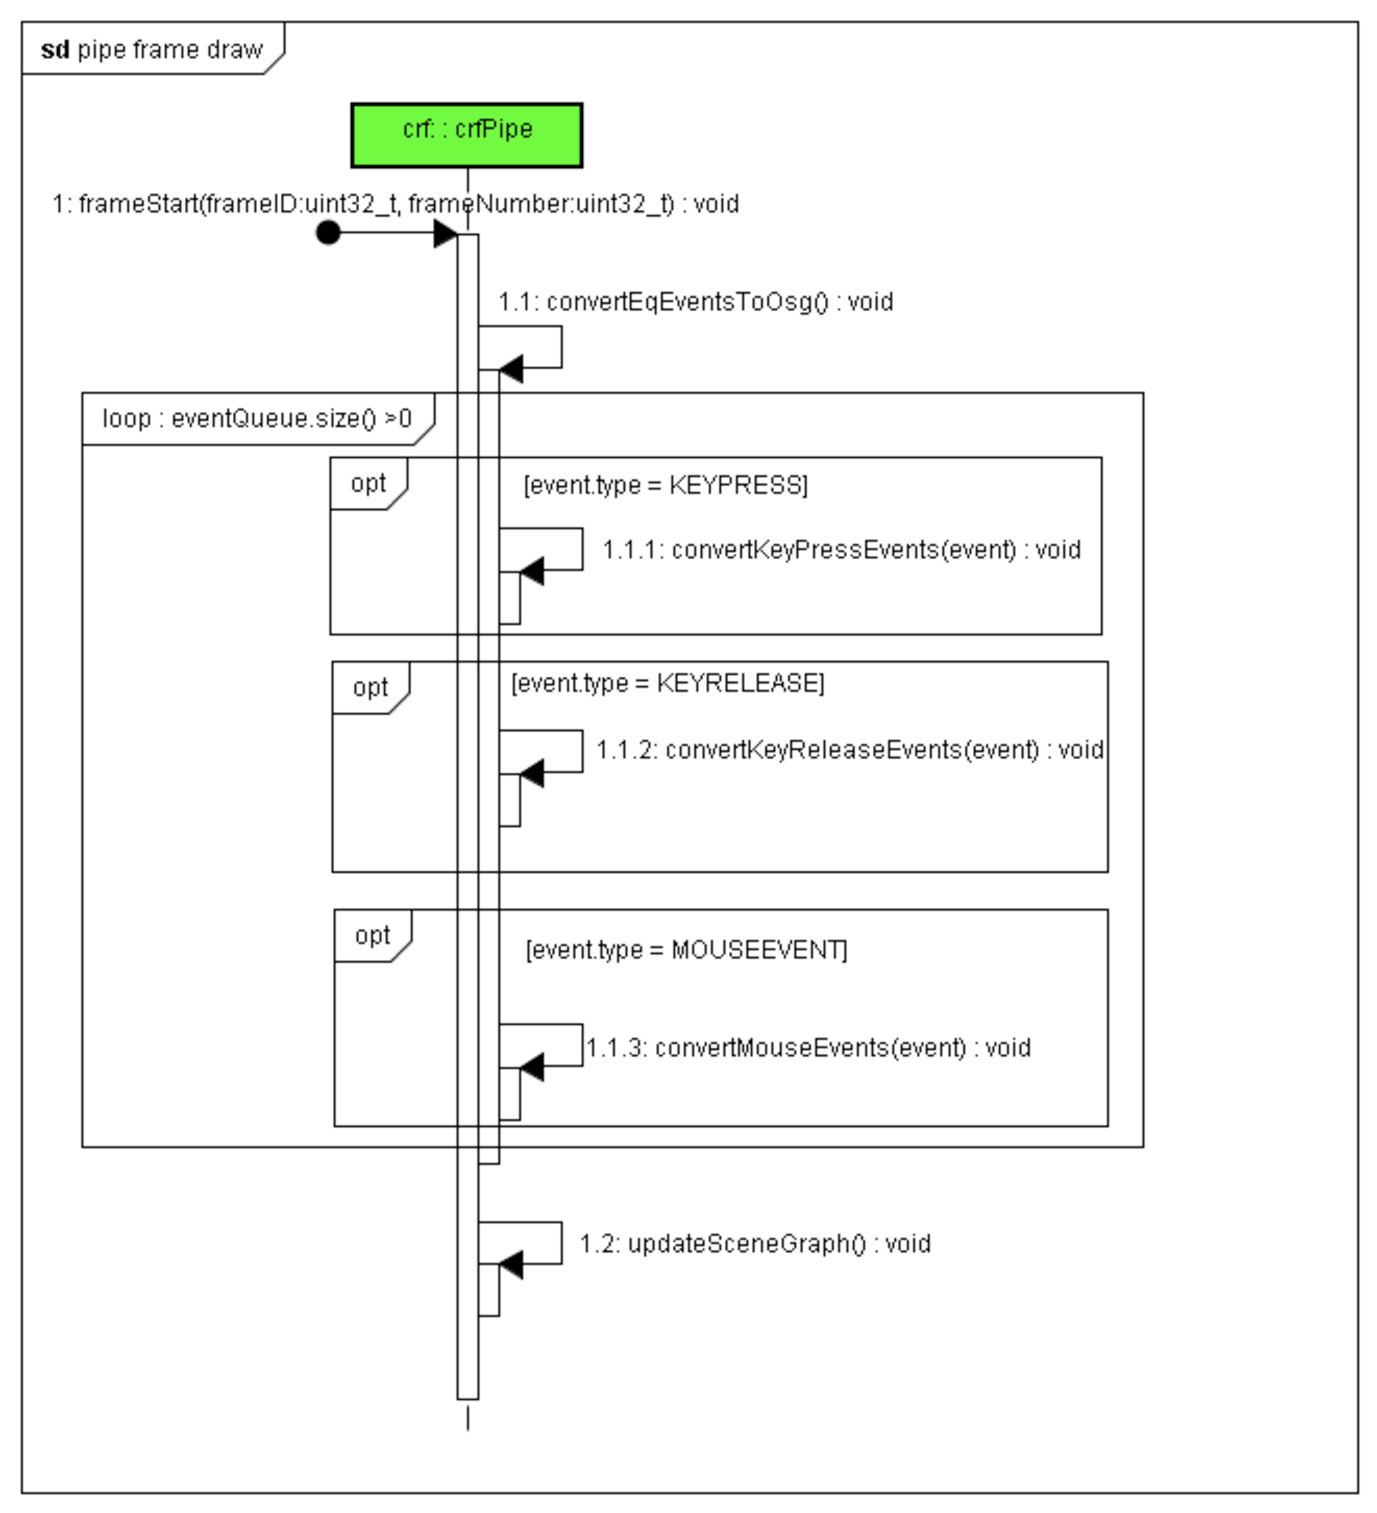
\includegraphics[width=0.70\textwidth]{../figures/crf_seq_pipe_frame_draw_01}
	\caption{the pipe's \texttt{frameDraw()} function as a sequence diagram }
	\label{fig:crf_seq_pipe_frame_draw_01}
\end{figure}

\section{Limitations}
\label{sec:crfLimitations}
\subsection{Scene Graph Creation}
Due to the fact that in Equalizer configurations with $n$ pipes on one node $n$ \gls{osg} scene graphs are created. The used objects in this creation-process must not be global and/or static. This is because every scene graph has to be completely independent and must not share the same memory. If static objects are used, every scene graph refers to the same memory on the node with several pipes. This causes errors or even segmentation faults.

\subsection{Dynamic Scene Graphs}
Changes in the scene graph have to be synchronised over all pipes and nodes. Due to the fact that distributed objects (the \texttt{FrameData} class at runtime and the \texttt{InitData} class on start-up in the \gls{crf}) provide the only way to communicate between pipes and nodes. 
%All scene graph changes have to be initiated due a distributed objects.
Common viewer bound \gls{osg} event handlers (like the \texttt{osgGA::TrackBallManipulator} or the \texttt{osgViewer::Statshandler}) can be used because the \gls{crf} sends all mouse and keyboard events to every viewer of every pipe with its \texttt{FrameData} class. 
To add other input devices like a 3D joystick or similar, the new events have to be pushed from the \texttt{Config} class over a distributed object to every pipe. Now, the scene graph's changes have to be made in the pipe. Due to the fact that the distributed objects are completely synchronised, every pipe receives the same events at the same time (frame). To summarise, all changes in a scene graph have to be caused by distributed data. In our case this responsibility is taken by the \texttt{FrameData} class.

\subsection{Model Loading with Multiple Pipes on One Machine}
Random segmentation faults occured when loading \gls{osg} models with \texttt{osgDB::loadNodeFile()} on a multipipe node with just one running instance of the CRF application. After some debugging efforts these random errors seem to be caused by a not thread-safe singleton pattern, used in \gls{osg}.
This error does not appear in multinode environments where on every node one instance of the \gls{crf} application runs per node and therefore the singleton pattern is processed properly.

\section{Previous Work}
This framework is based on the basic \gls{osg}-Equalizer application eqOSG, realised by a \gls{vr} research group of the University of Siegen. 

% Outlook
% ==========================================
% Thesis Report - Outlook ( all )
% ==========================================
\chapter{Outlook}

\section{Equalizer}

Two days ago the chief developer of Equalizer announced the Version 1.0 of Equalizer in the next few weeks/month. Our framework was developed and tested on top of Equalizer version 0.6-rc1. New features can be found at the official website of Equalizer: \href{http://www.equalizergraphics.com}{http://www.equalizergraphics.com}.

One of the changes of Equalizer that may affect our framework is the change of the configuration file formats. Equalizer writes on its website:

\begin{quote}
	Note that this format is the representation for the server's low-level scalable rendering engine. Eventually this file format will be replaced by a higher-level format or \gls{api}, and may even be partially hidden from the user. Automatic configuration and load balancing are not yet implemented, hence the need to have these low-level configuration files.
\end{quote}

As Equalizer 1.0 is considered to contain stable parts only, it would be a future objetive to upgrade it in the framework.

\section{CAVE Rendering Framework}
During our thesis project we could realise our main goal: An easy-to-use framework for the desired integration of OSG into Equalizer. To provide more possibilities, we expanded the framework with more functionality. But there are still a lot of possibilities to advance this project. We would like to point out some of these possible future enhancements.

\subsection{Distributed Objects}
At the moment, the CRF provides no simple mechanism to add more custom distributed data objects to the application. We could not find a simple approach to achieve this feature in a satisfying manor. A distributed object has to be mapped at both sides (master/slave) of the (network) application, committed, synced and counted which leads into a lot of changes just for this new object. To do this, one has to edit more or less all the CRF/eqOsg classes.

\subsection{Advanced Control Application}
Currently we cannot provide a specialised and advanced server application. It is a common approach in Equalizer for more complex applications to create an executable which does absolutely no rendering tasks but handles user input, physics (collision detection), haptics, data distribution or similar. Consult the \cite{eqPG} for further information about differences between client and server applications in Equalizer.

\subsection{Tracking}
It should not be a big deal to introduce a tracker into the CRF. Because of the fact that our key and mouse bound camera handling simulates a kind of tracker, it should be easy to add a real tracker. A straight forward approach would be to add a reference to the tracker's interface in the \texttt{crfConfig} class and thereafter pass the tracker's current head matrix to the Equalizer's head matrix in the \texttt{crfConfig::startFrame()} function. Of course this would bring along a lot of calibration work and some special requirements to the OSG scene graph, but technically it should be absolutely possible with the CRF. Unfortunately, there was not enough time to test this use case.

\subsection{Distributed OSG Scene Graph}
Another big effort would be needed to achieve a fully distributed \gls{osg} scene graph. A trial can be found in the community \cite{distOSG}, but this project has not been finished yet and is highly likely currently stopped. 

% Testing 
\chapter{Testing}

Automatisierte Tests f\"ur ein Framework im grafischen Bereich sind meist recht schwierig zu realisieren. Wir gehen davon aus, dass die verwendeten Frameworks Equalizer und SceneGraph (OSG oder OGRE) selbst schon getestet sind. Unsere Tests beschr\"anken sich also darauf, ob die Schnittstellen vom SceneGraph zu dem \textit{CAVE Rendering Framework} und von diesem zu Equalizer wie gew\"unscht funktionieren.

Nebst der korrekten Funktionsweise des Frameworks interessieren wir uns vor allem auch auf eine gute Performance. 

Um unsere Arbeit zu verifizieren, implementieren wir eine Testapplikation, mit deren Hilfe die Use Cases getestet werden k\"onnen.

\section{Testapplikationen}

Die Testapplikation muss im CAVE der BFH-TI lauff\"ahig sein. Folgende Funktionalit\"aten des Frameworks m\"ussen mithilfe der Testapplikation \"uberpr\"uft werden k\"onnen:

\begin{description}
\item[Modell] Aus der Applikation m\"ussen SG-Modelle geladen werden k\"onnen.
\item[Stereo Performance] Es muss eine M\"oglichkeit geben, die Performance von Stereobilder zu \"uberpr\"ufen.
\item[Shader] Das Framework sollte Shader-tauglich sein (Optionale Anforderung). Es sollten also verschiedene Shader geladen werden k\"onnen.
\item[Haptics] Falls Haptics im Framework bereits integriert wird (Optionale Anforderung), so muss es eine M\"oglichkeit geben, Haptics ein- und auszuschalten.
\end{description}

Grunds\"atzlich gilt, dass die Testapplikation eine Feature-by-Feature Applikation sein soll, d.h. f\"ur jedes Implementierte Feature im Framework soll es einen Test Case geben der (dynamisch) ein- und ausgeschaltet werden kann.

Falls eine geeignete bestehende Applikation gefunden werden kann, mit deren Hilfe die Features getestet werden k\"onnen, so kann auch diese verwendet werden.

\section{Test Cases}
Um eine m\"oglichst komplette und dokumentierte Testumgebung zu erlangen, soll zu jedem implementierten Feature des Frameworks ein Test Case formuliert werden. Dieser soll nebst dem Test Szenario auch dessen Pre- und Postconditions enthalten.
Wichtig ist, dass das Testing iterativ erfolgt und wo m\"oglich. Tests, die oft ausgef\"uhrt werden sollen, sollten wenn m\"oglich automatisiert werden. Grunds\"atzlich sollte immer ersichtlich sein, was getestet wird, damit zum Schluss eine vollst\"andige Liste von Tests ersichtlich ist.

% Demo / Test Applications - all
% ==========================================
% Technical Report - Demo Applications ( all )
% ==========================================
\chapter{Demo Applications}

The \gls{crf} package comes with some demo applications to demonstrate the functionalities of the framework. The following list gives an overview of these applications and their purpose:

\begin{description}
	\item[\texttt{crfHelloWorld}]\hfill\\
		The purpose of this very simple application is to test if the CRF is installed and running properly. Since it is a very slim and simple application, it can be used to test Equalizer configuration files. The application simply shows the word \texttt{OSG} written in light blue flickering letters. One can load any desired \texttt{*.osg} model files by adding the following parameter: \texttt{--model=<filename>}. Screenshots can be found in the Appendix \ref{sec:appendixHelloWorld}.
	\item[\texttt{crfShaderDemo}]\hfill\\
		The sole purpose of this demo application is to verify whether \gls{glsl} shaders can be loaded and executed. It shows the same shader demo provided by the \gls{osg} group.
	\item[\texttt{crfSpaceFlight}]\hfill\\
		This last demo application shows some planets rotating around the sun.
\end{description}

Appendix \ref{sec:appendixDemo} holds screenshots of the expected output for each application.


% =======================================
% Acronyms
% =======================================
\addcontentsline{toc}{chapter}{Glossary}
\printglossary[title={Glossary}]

% =======================================
% Bibliography
% =======================================
\addcontentsline{toc}{chapter}{Bibliography}
\bibliography{../tex-include/crfbibliography} % Note the lack of whitespace between the commas and the next bib file.

% =======================================
% Appendices
% =======================================
%\addcontentsline{toc}{chapter}{Appendices}
\appendix

\chapter{Worklog}
\label{sec:appendixWorklog}

\begin{table}[H]
	\centering
	\begin{tabular}{|b{0.1\textwidth}|p{0.3\textwidth}|p{0.1\textwidth}|p{0.1\textwidth}|p{0.23\textwidth}|}
		\hline \multicolumn{2}{|l|}{\color{red}{\bfseries 16.02.2009}} & \multicolumn{3}{l|}{\color{red}{\bfseries Project Start}} \\
		\hline
		\hline \bfseries week 1-2 & \multicolumn{4}{l|}{\bfseries 16.02.2009 - 26.02.2009} \\
		\hline
		\hline \bfseries who? & \bfseries what? & \bfseries output & \bfseries achieved & \bfseries comment \\ 
		\hline hullb2 & Equalizer knowledge & running Equalizer installation & \tick & \quad\quad- \\
		\hline waltj3 / brods1 & OSG/OGRE setup & \quad\quad- & \tick & \quad\quad- \\
		\hline all & index for requirement specification & \quad\quad- & \tick & \quad\quad- \\ 
		\hline
	\end{tabular}
	\caption{Worklog Week 1-2: 16.02.2009 - 26.02.2009}
\end{table}

\begin{table}[H]
	\centering
	\begin{tabular}{|b{0.1\textwidth}|p{0.3\textwidth}|p{0.1\textwidth}|p{0.1\textwidth}|p{0.23\textwidth}|}
		\hline \bfseries week 3 & \multicolumn{4}{l|}{\bfseries 27.02.2009 - 05.03.2009} \\
		\hline
		\hline \bfseries who? & \bfseries what? & \bfseries output & \bfseries achieved & \bfseries comment \\ 
		\hline all & Prototypes & \quad\quad- & \tick & \quad\quad- \\
		\hline all & eqOSG evaluation & \quad\quad- & \tick & \quad\quad- \\
		\hline all & eqOGRE evaluation & \quad\quad- & \tick & \quad\quad- \\
		\hline all & first draft of requirements specification & \quad\quad- & \tick & \quad\quad- \\
		\hline
	\end{tabular}
	\caption{Worklog Week 3: 27.02.2009 - 05.03.2009}
\end{table}

\begin{table}[H]
	\centering
	\begin{tabular}{|b{0.1\textwidth}|p{0.3\textwidth}|p{0.1\textwidth}|p{0.1\textwidth}|p{0.23\textwidth}|}
		\hline \bfseries week 4 & \multicolumn{4}{l|}{\bfseries 06.03.2009 - 12.03.2009} \\
		\hline
		\hline \bfseries who? & \bfseries what? & \bfseries output & \bfseries achieved & \bfseries comment \\ 
		\hline all & requirements specification finished & \quad\quad- & \tick & \quad\quad- \\
		\hline
		\hline all & \multicolumn{4}{l|}{\color{red}{\bfseries 13.03.09: Appointment with Expert: H. van der Kleij}} \\
		\hline
	\end{tabular}
	\caption{Worklog Week 4: 06.03.2009 - 12.03.2009}
\end{table}


\begin{table}[H]
	\centering
	\begin{tabular}{|b{0.1\textwidth}|p{0.3\textwidth}|p{0.1\textwidth}|p{0.1\textwidth}|p{0.23\textwidth}|}
		\hline \bfseries week 5 & \multicolumn{4}{l|}{\bfseries 13.03.2009 - 19.03.2009} \\
		\hline
		\hline \bfseries who? & \bfseries what? & \bfseries output & \bfseries achieved & \bfseries comment \\ 
		\hline all & corrections of requirements specification & \quad\quad- & \tick & \quad\quad- \\
		\hline
		\hline \color{red}{\bfseries M1} & \multicolumn{2}{l|}{\color{red}{\bfseries Functional specification}} & \tick & \quad\quad- \\
		\hline \color{red}{\bfseries M2} & \multicolumn{2}{l|}{\color{red}{\bfseries Prototype finished}} & \tick & \quad\quad- \\
		\hline
	\end{tabular}
	\caption{Worklog Week 5: 13.03.2009 - 19.03.2009}
\end{table}


\begin{table}[H]
	\centering
	\begin{tabular}{|b{0.1\textwidth}|p{0.3\textwidth}|p{0.1\textwidth}|p{0.1\textwidth}|p{0.23\textwidth}|}
		\hline \bfseries week 6 & \multicolumn{4}{l|}{\bfseries 20.03.2009 - 26.03.2009} \\
		\hline
		\hline \bfseries who? & \bfseries what? & \bfseries output & \bfseries achieved & \bfseries comment \\ 
		\hline all & Evaluate scene graph techniques & \quad\quad- & \tick & \quad\quad- \\
		\hline
	\end{tabular}
	\caption{Worklog Week 6: 20.03.2009 - 26.03.2009}
\end{table}

\begin{table}[H]
	\centering
	\begin{tabular}{|b{0.1\textwidth}|p{0.3\textwidth}|p{0.1\textwidth}|p{0.1\textwidth}|p{0.23\textwidth}|}
		\hline \bfseries week 7 & \multicolumn{4}{l|}{\bfseries 27.03.2009 - 02.04.2009} \\
		\hline
		\hline \bfseries who? & \bfseries what? & \bfseries output & \bfseries achieved & \bfseries comment \\ 
		\hline all & Eurographics 2009 & \multicolumn{3}{l|}{networking with other interested people} \\
		\hline
	\end{tabular}
	\caption{Worklog Week 7: 27.03.2009 - 02.04.2009}
\end{table}

\begin{table}[H]
	\centering
	\begin{tabular}{|b{0.1\textwidth}|p{0.3\textwidth}|p{0.1\textwidth}|p{0.1\textwidth}|p{0.23\textwidth}|}
		\hline \bfseries week 8 & \multicolumn{4}{l|}{\bfseries 03.04.2009 - 09.04.2009} \\
		\hline
		\hline \bfseries who? & \bfseries what? & \bfseries output & \bfseries achieved & \bfseries comment \\ 
		\hline all & holidays & \quad\quad- & \quad\quad- & \quad\quad- \\
		\hline
	\end{tabular}
	\caption{Worklog Week 8: 03.04.2009 - 09.04.2009}
\end{table}

\begin{table}[H]
	\centering
	\begin{tabular}{|b{0.1\textwidth}|p{0.3\textwidth}|p{0.1\textwidth}|p{0.1\textwidth}|p{0.23\textwidth}|}
		\hline \bfseries week 9 & \multicolumn{4}{l|}{\bfseries 10.04.2009 - 16.04.2009} \\
		\hline
		\hline \bfseries who? & \bfseries what? & \bfseries output & \bfseries achieved & \bfseries comment \\ 
		\hline waltj3 & Integration eqPly und OSG & \quad\quad- & \tick & \quad\quad- \\
		\hline hullb2 / brods1 & Compilation of CAVE clone & CAVE Clone & \tick & \quad\quad- \\
		\hline hullb2 / brods1 & Setup Ubuntu \& Windows Vista on CAVE Clone & CAVE clone ready & \tick & \quad\quad- \\
		\hline hullb2 & 1 node N pipe config & config files & \tick & problems with windows configs \\
		\hline hullb2 & config files for Windows & config files & \cross & multipipe config for Windows Vista not possible \\
		\hline
	\end{tabular}
	\caption{Worklog Week 9: 10.04.2009 - 16.04.2009}
\end{table}

\begin{table}[H]
	\centering
	\begin{tabular}{|b{0.1\textwidth}|p{0.3\textwidth}|p{0.1\textwidth}|p{0.1\textwidth}|p{0.23\textwidth}|}
		\hline \bfseries week 10 & \multicolumn{4}{l|}{\bfseries 17.04.2009 - 23.04.2009} \\
		\hline
		\hline \bfseries who? & \bfseries what? & \bfseries output & \bfseries achieved & \bfseries comment \\ 
		\hline hullb2 & Equalizer Configs for CAVE Server & configuration files & \tick & \quad\quad- \\
		\hline waltj3 & Integration eqPly and OSG & \quad\quad- & \tick & \quad\quad- \\
		\hline brods1 & CMake & CMake build scripts & \tick & \quad\quad- \\
		\hline
	\end{tabular}
	\caption{Worklog Week 10: 17.04.2009 - 23.04.2009}
\end{table}

\begin{table}[H]
	\centering
	\begin{tabular}{|b{0.1\textwidth}|p{0.3\textwidth}|p{0.1\textwidth}|p{0.1\textwidth}|p{0.23\textwidth}|}
		\hline \bfseries week 11 & \multicolumn{4}{l|}{\bfseries 24.04.2009 - 30.04.2009} \\
		\hline
		\hline \bfseries who? & \bfseries what? & \bfseries output & \bfseries achieved & \bfseries comment \\ 
		\hline hullb2 & planning until May & agenda & \tick & \quad\quad- \\
		\hline hullb2 / brods1 & 3D stereo tests with eqOSG & \quad\quad- & \tick & \quad\quad- \\
		\hline hullb2 / brods1 & network rendering: terminology server/client, tests & \quad\quad & \cross & terminology OK, network tests successful on private setup, but failed in CAVE \\
		\hline hullb2 / waltj3 & CAVE 4-pipe Setup: Hardware config & config file & \tick & \quad\quad- \\
		\hline hullb2 / brods1 & CAVE 4-pipe Setup: Software config & config file & \tick & \quad\quad- \\
		\hline waltj3 & Eventhandling with eqOSG & \quad\quad -  & \tick & \quad\quad- \\
		\hline waltj3 & Define CRF Structure & Index & \quad\quad\color{yellow}{\bfseries!} & partially done \\
		\hline brods1 & Templates for documentation & templates & \quad\quad\color{yellow}{\bfseries!} & partially done \\
		\hline
	\end{tabular}
	\caption{Worklog Week 11: 24.04.2009 - 30.04.2009}
\end{table}

\begin{table}[H]
	\centering
	\begin{tabular}{|b{0.1\textwidth}|p{0.3\textwidth}|p{0.1\textwidth}|p{0.1\textwidth}|p{0.23\textwidth}|}
		\hline \bfseries week 12 & \multicolumn{4}{l|}{\bfseries 01.05.2009 - 07.05.2009} \\
		\hline
		\hline \bfseries who? & \bfseries what? & \bfseries output & \bfseries achieved & \bfseries comment \\ 
		\hline brods1 & Concept for Demo App & \quad\quad- & \tick & \quad\quad- \\
		\hline all & Concept for all documents & Index & \tick & \quad\quad- \\
		\hline brods1 & Templates for documentation & templates & \tick & \quad\quad- \\
		\hline waltj3 & Test protocols & protocols & \cross & \quad\quad- \\
		\hline waltj3 & Eventhandling & - & \tick& \quad\quad-\\
		\hline hullb2 & network rendering in CAVE & \quad\quad- & \cross & did not work yet. In contact with community \\
		\hline waltj3 & class diagram for CRF & diagram & \tick & \quad\quad- \\
		\hline 
	\end{tabular}
	\caption{Worklog Week 12: 01.05.2009 - 07.05.2009}
\end{table}

\begin{table}[H]
	\centering
	\begin{tabular}{|b{0.1\textwidth}|p{0.3\textwidth}|p{0.1\textwidth}|p{0.1\textwidth}|p{0.23\textwidth}|}
		\hline \bfseries week 13 & \multicolumn{4}{l|}{\bfseries 08.05.2009 - 14.05.2009} \\
		\hline
		\hline \bfseries who? & \bfseries what? & \bfseries output & \bfseries achieved & \bfseries comment \\ 
		\hline hullb2 / brods1 & First version of demo app & demo app & \tick & \quad\quad- \\
		\hline brods1 & Replace Windows Vista with Windows XP & Windows XP setup & \tick & Equalizer did not work properly on Windows Vista \\
		\hline waltj3 & first working CRF & crf & \tick & \quad\quad- \\
		\hline waltj3 & eqOSG problems solved & \quad\quad- & \tick & \quad\quad- \\
		\hline hullb2 & sample document for documentation & \quad\quad- & \tick & \quad\quad- \\
		\hline
	\end{tabular}
	\caption{Worklog Week 13: 08.05.2009 - 14.05.2009}
\end{table}

\begin{table}[H]
	\centering
	\begin{tabular}{|b{0.1\textwidth}|p{0.3\textwidth}|p{0.1\textwidth}|p{0.1\textwidth}|p{0.23\textwidth}|}
		\hline \bfseries week 14 & \multicolumn{4}{l|}{\bfseries 15.05.2009 - 21.05.2009} \\
		\hline
		\hline \bfseries who? & \bfseries what? & \bfseries output & \bfseries achieved & \bfseries comment \\ 
		\hline brods1 & Concept for user manual & Concept & \tick & \quad\quad- \\
		\hline hullb2 / waltj3 & 80\% of Technical Documentation & Tech. Doc. & \quad\quad\color{yellow}{\bfseries !} & About 50\% finished \\
		\hline
	\end{tabular}
	\caption{Worklog Week 14: 15.05.2009 - 21.05.2009}
\end{table}

\begin{table}[H]
	\centering
	\begin{tabular}{|b{0.1\textwidth}|p{0.3\textwidth}|p{0.1\textwidth}|p{0.1\textwidth}|p{0.23\textwidth}|}
		\hline \bfseries week 15 & \multicolumn{4}{l|}{\bfseries 22.05.2009 - 28.05.2009} \\
		\hline
		\hline \bfseries who? & \bfseries what? & \bfseries output & \bfseries achieved & \bfseries comment \\ 
		\hline hullb2 / brods1 & Major features integrated in demo app & \quad\quad- & \quad\quad\color{yellow}{\bfseries !} & development of demo app not forced. Feature-by-Feature app implemented instead. \\
		\hline waltj3 / hullb2 & Testcases & Excel sheet with testcases & \tick & \quad\quad- \\
		\hline all & Technical Documentation finished & Documentation & \quad\quad\color{yellow}{\bfseries !} & About 80\% done \\
		\hline all & 80\% of Thesis Documentation & Thesis Documentation & \quad\quad\color{yellow}{\bfseries !} & About 20\% done \\
		\hline waltj3 & Framework finished & CRF & \quad\quad\color{yellow}{\bfseries !} & open test cases to pass \\
		\hline
		\hline \color{red}{\bfseries M3} & \multicolumn{2}{l|}{\color{red}{\bfseries Development finished}} & \tick & \quad\quad- \\
		\hline
	\end{tabular}
	\caption{Worklog Week 15: 22.05.2009 - 28.05.2009}
\end{table}

\begin{table}[H]
	\centering
	\begin{tabular}{|b{0.1\textwidth}|p{0.3\textwidth}|p{0.1\textwidth}|p{0.1\textwidth}|p{0.23\textwidth}|}
		\hline \bfseries week 16 & \multicolumn{4}{l|}{\bfseries 29.05.2009 - 04.06.2009} \\
		\hline
		\hline \bfseries who? & \bfseries what? & \bfseries output & \bfseries achieved & \bfseries comment \\ 
		\hline all & all documents finished & documents & \quad\quad\color{yellow}{\bfseries !} & first draft finished, sent to expert and supervisors \\
		\hline hullb2 / brods1 & Demo App finished & \quad\quad- & \tick & running demo app and running feature by feature app \\
		\hline brods1 & Stress Test application & working app & \tick & \quad\quad- \\
		\hline waltj3 / hullb2 & Testcases in CAVE & passed tests & \tick & \quad\quad- \\
		\hline brods1 & CMake script for delivery & CMake Script & \tick & \quad\quad- \\
		\hline
	\end{tabular}
	\caption{Worklog Week 16: 29.05.2009 - 04.06.2009}
\end{table}


\begin{table}[H]
	\centering
	\begin{tabular}{|b{0.1\textwidth}|p{0.3\textwidth}|p{0.1\textwidth}|p{0.1\textwidth}|p{0.23\textwidth}|}
		\hline \bfseries week 17 & \multicolumn{4}{l|}{\bfseries 05.06.2009 - 11.06.2009} \\
		\hline
		\hline \bfseries who? & \bfseries what? & \bfseries output & \bfseries achieved & \bfseries comment \\ 
		\hline brods1 & Bash Scripts for delivery & scripts & \tick & \quad\quad- \\
		\hline hullb2 / waltj3 & final tests & \quad\quad- & \tick & \quad\quad- \\
		\hline all & final review of documentation & \quad\quad- & \tick & \quad\quad- \\
		\hline hullb2 & A4 page for Bachelor Book & A4 page & \tick & \quad\quad- \\
		\hline brods1 & CDs with source code for delivery & CDs & \tick & \quad\quad- \\
		\hline hullb2 & Printing documentation & 5 hardcopies & \tick & \quad\quad- \\
		\hline all & Delivery of hardcopies & \quad\quad- & \tick & \quad\quad- \\
		\hline
		\hline \color{red}{\bfseries M4} & \multicolumn{2}{l|}{\color{red}{\bfseries Tests finished}} & \tick & \quad\quad- \\
		\hline
		\hline \multicolumn{2}{|l|}{\color{red}{\bfseries 16.02.2009}} & \multicolumn{3}{l|}{\color{red}{\bfseries Project End}} \\
		\hline
	\end{tabular}
	\caption{Worklog Week 17: 05.06.2009 - 11.06.2009}
\end{table}






%\printglossaries

\end{document}
